\documentclass[11pt]{scrartcl}
\usepackage{color}
%\usepackage{enumitem}
%\setlist[itemize,2]{label=\textbullet}
\usepackage{geometry}
\geometry{a4paper, top=25mm, left=20mm, right=20mm, bottom=40mm, headsep=10mm, footskip=5mm}
\usepackage{ucs}
\usepackage[utf8x]{inputenc}
%\usepackage{german}
\usepackage{soul}
\usepackage{amsmath,amssymb,amstext}
\usepackage{graphicx}
\usepackage[automark]{scrpage2}
\usepackage{subcaption}
\usepackage{footnote}
\makesavenoteenv{tabular} %make footnotes in tables and tabulars appear
\makesavenoteenv{table}
%\usepackage{caption}
%\usepackage{subfigure}
%\usepackage{subfig}

\usepackage{algpseudocode,algorithm,algorithmicx}
\newcommand*\DNA{\textsc{dna}}

\newcommand*\Let[2]{\State #1 $\gets$ #2}
\algrenewcommand\algorithmicrequire{\textbf{Precondition:}}
\algrenewcommand\algorithmicensure{\textbf{Postcondition:}}

\usepackage[ngerman]{babel} 
\usepackage{xspace}
\usepackage{hyperref}
%\RequirePackage[ngerman=ngerman-x-latest]{hyphsubst}
\newcommand{\Gu}{\glqq{}}		%Gänsefüßchen unten
\newcommand{\Go}{\grqq\xspace} 
\newcommand{\red}{\textcolor{red}}
\newcommand{\ita}{\item[$\rightarrow$]}
\DeclareSymbolFont{matha}{OML}{txmi}{m}{it}% txfonts
\DeclareMathSymbol{\varv}{\mathord}{matha}{118}
\renewcommand*\labelitemii{-}
%\newcommand{\tightemize}{\vspace{-2mm}\begin{itemize}\setlength\itemsep{0em}}
\pagestyle{scrheadings}
\pagenumbering{arabic}	        %Gänsefüßchen oben
 \addtolength{\textheight}{25mm}
%\title{Lernende und Planende Roboter}
%\author{Sophie v. Schmettow}
%\date{\today{} in Karlsruhe}

\begin{document}

%----------------------------------------------------------------------------------------
%	TITLE PAGE
%----------------------------------------------------------------------------------------
\begin{titlepage}

\begin{center}


% Upper part of the page

\includegraphics[width=0.4\textwidth]{Logo_KIT.png}\\[1cm]    



\textsc{\Large Zusammenfassung}\\[0.5cm]


% Title
{ \huge \bfseries Mensch Maschine Interaktion}\\[0.4cm]
{ \large \bfseries Institut für Telematik -- Lehrstuhl für Pervasive Computing Systems}
\bigskip

% Author and supervisor

Sophie \textsc{v. Schmettow}\\
SoSe 16\\



\vfill

% Bottom of the page
{\large \today{} in Karlsruhe} 

\end{center}


\end{titlepage}

%----------------------------------------------------------------------------------------
%	ARTICLE CONTENTS
%----------------------------------------------------------------------------------------

\tableofcontents
\newpage

%----------------------------------------------------------------------------------------
%	UTILS
%----------------------------------------------------------------------------------------

%\begin{figure*}[ht]\centering % Using \begin{figure*} makes the figure take up the entire width of the page
%\includegraphics[width=\linewidth]{view}
%\caption{Wide Picture}
%\label{fig:view}
%\end{figure*}



%\begin{equation}
%\cos^3 \theta =\frac{1}{4}\cos\theta+\frac{3}{4}\cos 3\theta
%\label{eq:refname2}
%\end{equation}



%\begin{enumerate}[noitemsep] % [noitemsep] removes whitespace between the items for a compact look
%\item First item in a list
%\item Second item in a list
%\item Third item in a list
%\end{enumerate}



%\begin{figure}[ht]\centering
%\includegraphics[width=\linewidth]{results}
%\caption{In-text Picture}
%\label{fig:results}
%\end{figure}

%Reference to Figure \ref{fig:results}.


%\begin{table}[hbt]
%\caption{Table of Grades}
%\centering
%\begin{tabular}{llr}
%\toprule
%\multicolumn{2}{c}{Name} \\
%\cmidrule(r){1-2}
%First name & Last Name & Grade \\
%\midrule
%John & Doe & $7.5$ \\
%Richard & Miles & $2$ \\
%\bottomrule
%\end{tabular}
%\label{tab:label}
%\end{table}



%\begin{description}
%\item[Word] Definition
%\item[Concept] Explanation
%\item[Idea] Text
%\end{description}

%----------------------------------------------------------------------------------------
%	ARTICLE CONTENTS
%----------------------------------------------------------------------------------------

\section*{Disclaimer}
Dieses Dokument wurde im Rahmen des Master-Studiums
für das Modul \glqq Mensch-Maschine-Interaktion\grqq{} erstellt. Es stellt eine 
Zusammenfassung dar und dient zur Vorbereitung auf die
mündliche Prüfung. Neben den Materialien der Vorlesung
fließen auch weitere Quellen ein, um den behandelten Stoff
auszuarbeiten. Auf den Verweis von Quellen wird verzichtet,
da die Erstellung keinerlei wissenschaftlichen Zweck verfolgt
und nur für den privaten Gebrauch bestimmt ist.


%Lecture Content Overview (VL1, F24):
%1) Basics of Cognitive Science
%- Human Information Processing
%- Perception
%2) Formative Design and Evaluation of Human Computer Interaction (HCI)
%- Methods and Tools for Design
%3) Summative Evaluation of HCI
%- Basics of Human Studies and Statistics for Studies
%4) Best Practice in HCI
%- Concepts, Models, Guidelines, Methods

\section{Introduction} %(1. VL)
\subsection{Definitionen}
\begin{itemize}
	\item \textbf{Pervasive Computing}
	\begin{itemize}
		\item Pervasive Computing $\approx$ Ubiquitous Computing
		\item pervasive = \textit{alles durchdringend}
		\item IBM-Definition: \glqq Convenient access, through a new class of appliances, to relevant information with the ability to easily take action on it when and where you need\grqq
		\item Beispiel: Smartphones $\rightarrow$ relativ neue Technologie, daher viel höhrere Dynamik in der Entwicklung als beim Desktop. 
		\item Implizite Interaktionen: Gerät reagiert implizit auf User-Aktivität (insbesondere bei Smart Homes), jüngere lernen das besser (je älter man wird, desto mehr muss man anhand von Bezügen zu bereits Gelerntem/Metaphern lernen)
	\end{itemize}
	\item \textbf{Human Adopted Production}
	\begin{itemize}
		\item Comber and Maltby (1997) found that both overly simple and overly complex computing interfaces were low in usability 
		\item Wie kann man den User \glqq bei Laune halten\grqq ?\\
	 	$\rightarrow$ Die aktuell erfahrene Komplexität muss im Mittelmaß sein\\
	 	$\rightarrow$ Lernsysteme greifen per GSR Stress Level des Users ab und tunen dementsprechend das Lernsystem\\
	 	$\rightarrow$ kognitive Paramater sind sehr individuell
		\begin{figure}[h!]
			\centering
			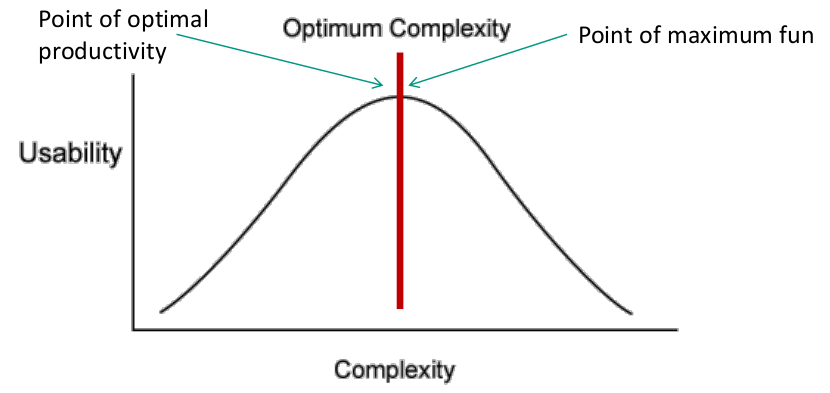
\includegraphics[width=.4\textwidth]{img/ch01_HAP.png}
			\caption{Human Adopted Production}
			\label{HAP}
		\end{figure} 
	\end{itemize}
	\item \textbf{Mensch-Maschine Interaktion}
	\begin{itemize}
		\item Important part of Pervasive Computing, e.g. Mobile Phone interfaces
		\item Pervasive Computing Technology produces now most/all innovative human machine interfaces, e.g. augmented reality glasses
	\end{itemize}
\end{itemize}
\subsection{Anwendungen}
\begin{itemize}
	\item Reprogramming Senses: Proxmity Helmet (mit Arduino) $\rightarrow$ wird nach einer Weile zum Gefühl, so kann man neue Sinne erschaffen
	\item Augmented Reality, Mobile Computing User Interface Software Design
	\item Wearable Thermography: detektiert Überbelastung bei Sport...
	\item Ubiquitous Sensing: Lobster House, Büro welches sich nach Sonne dreht, jeder Quadratmeter individuell klimatisierbar
\end{itemize}





\section{Evaluation/Observation}
There are two basic classes / times for studies and evaluation (and many variants):
\begin{itemize}
\item \textbf{Formative}: At the beginning to inform about context and to study possible options
\item \textbf{Summative}: To judge on the impact of a HCI design.
A summative evaluation of a design might be a
formative one for the next step.
\end{itemize}
\textbf{Evaluation}: Iterative design \& evaluation is a continuous process that examines:
\begin{itemize}
\item Why to evaluate: to check users’ requirements and that they can use the product and they like it.
\item What to evaluate: a conceptual model, early prototypes of a new system and later, more complete prototypes.
\item Where to evaluate: in natural and laboratory settings.
\item When to evaluate: Formative: throughout design; Summative: finished products can be evaluated to collect information to inform new products.
\end{itemize}
\textbf{Usability}: The extent to which a product can be used by specified users to achieve specified goals with \textbf{effectiveness, efficiency and satisfaction} in a specified context of use (\autoref{usab}).\\
 Over-arching usability principles: \textbf{Learnability, effectiveness, accommodation} for its intended user population.\\
 \begin{figure}[h!]
			\centering
			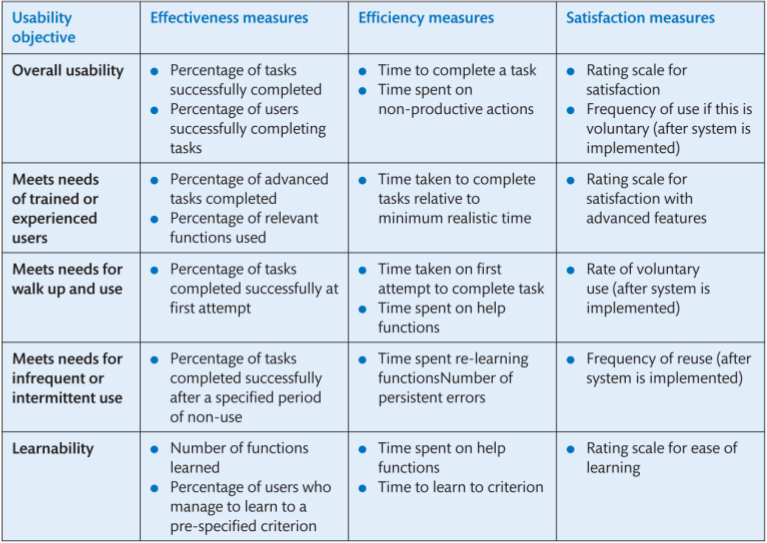
\includegraphics[width=\textwidth]{img/ch01_usab.png}
			\caption{What do we want to know -- Common usability metrics}
			\label{usab}
		\end{figure} 
\textbf{Evaluation classes}:
\begin{itemize}
\item \textbf{Setting}:
\begin{itemize}
\item Controlled settings: Setting conditions are controlled; non-controllable conditions are measured; e.g. Lab experiments, living labs
\item Natural settings: Study in ``everyday'' and natural conditions that cannot be controlled; some, but not all non-controllable conditions can be measured; e.g. Field studies, in-the-wild studies
\end{itemize}
\item \textbf{Evaluation Time}:
\begin{itemize}
\item Inspective: Inspection / Evaluation while run of an experiment or while use
\item Retrospective: Evaluation after run of the experiment or after use
\item Short term
\item Long term
\end{itemize}
\item \textbf{Partner}:
\begin{itemize}
\item The user: Gives direct feedback e.g. for use; Best for gaining new insight into context (If its an experiment: called ``subject'')
\item The expert: Allows for best practice information; Reported expert experience may require many users / test subjects to be collected
\end{itemize}
\item \textbf{Result type}:
\begin{itemize}
\item Subjective: Results cannot be directly compared between subjects
\item Objective Results can be directly compared between subjects (e.g. using statistics)
\item Quantitative: Results are numbers
\item Qualitative: Results are text
\end{itemize}
\end{itemize}
\textbf{Example Methods}:
\begin{itemize}
\item Inspective, End User Focused:
\begin{itemize}
\item Subjective Short Session: Think Aloud
\item Objective Short Session: Measurements of Workload, Interaction Process (e.g. Video Recording in User Setting / Usability Lab; Eye Gaze which is a quantitative/objective measure)
\item Subjective Long Session: Diary (Logging, asking questions from time to time e.g. through pop ups)
\end{itemize}
\item Inspective, Expert Focused: Cognitive Walk Through
\item Retrospective, End User Focused: Interviewing / Questionnaire
\end{itemize}
\textbf{Data Gathering -- Key Issues}
\begin{enumerate}
\item Setting goals: Decide how to analyze data once collected
\item Identifying participants: Decide who to gather data from
\item Relationship with participants: Clear and professional; Informed consent when appropriate
\item Triangulation: Look at data from more than one perspective; Collect more than one type of data, e.g. qualitative from experiments and qualitative from interviews.
\item Pilot studies: Small trial of main study
\end{enumerate}
\subsection{Data Gathering -- Interviews \& Questionnaires}
\textbf{Types of interviews}:
\begin{itemize}
\item \textbf{structured interviews}: pre-developed questions, strictly following the wording (e.g. introduction, purpose of the questionnaire); easy to carry out – but limited to the question set; more precise to evaluate
\item \textbf{semi-structured interviews}: structured part + ``open'' questions (``Tell me your ideas on ...'')
\item \textbf{unstructured interviews}: used e.g. when little background information is available; minimizes the influence of the questioner
\end{itemize}
Questionnaires: 
\begin{itemize}
\item Questions have orders (positive or negative, can be mixed)
\item Version needs to be adapted to population.
\item Instructions of use need to be clear.
\item No excess whitespace, not too long, no compound sentences or jargon.
\item frame: consent form, (monetary) compensation, time constraints, number of participants, introduction to scenario, scale type
\end{itemize}
Question and response format:
\begin{itemize}
\item Yes’ and ‘No’ checkboxes
\item Checkboxes that offer many options
\item Rating scales: Likert scales (5-point scale, \textit{strongly agree, agree, neutral, disagree, strongly disagree} $\rightarrow$ quantitative result), semantic scales
\item Open-ended responses
\end{itemize}
Conducting the interview:
\begin{itemize}
\item contextual factors (light, noise...) should be kept constant, interviewer should provide a neutral attitude, interviewee might try to say what he thinks you want to hear $\rightarrow$ questions to cross-check answers needed
\item[1.] Introduction: introduce yourself, explain the goals of the interview, reassure about the ethical issues, ask to record, present the informed consent form.
\item[2.] Warm-up: make first questions easy and non-threatening.
\item[3.] Main body: present questions in a logical order.
\item[4.] A cool-off period: include a few easy questions to defuse tension at the end.
\item[5.] Closure: thank interviewee, signal the end, e.g. switch recorder off.
\item documentation: notes, video taping, audio recording, photographs (always use visual impression)
\item interview can be enriched by props, e.g. prototype scenario
\item encouraging good responses: clarify purpose of study, promise anonymity, ensure questionnaire is well designed, Follow-up with emails/phone calls/letters, provide an incentive
$\rightarrow$ 40\% response rate is good, 20\% is often acceptable
\end{itemize}
Standard Questionnaires in HCI:
\begin{itemize}
\item System Usability Scale (SUS)
\item NASA Task Load Index (TLX)
\item Questionnaire for User Interface Satisfaction (QUIS)
\item Computer System Usability Questionnaire (CSUQ)
\end{itemize}
\textbf{System Usability Scale (John Brooke, 1986 for Digital Equipment) }
\begin{itemize}
\item Quick and dirty subjective measurement of usability in terms of Effectiveness, Efficiency and Satisfaction
\item Used for hardware, software, mobile devices, websites, applications
\item Evaluation: Positive questions get a 0-4 rating, negative ones a 4-0 rating, points are added and multiplied by 2.5 -- good result if over 68 (max: 100)
\item Benefits: Very easy scale (Likert); Useful in small sample sizes with o.k. results; Validity o.k. (you see differences in bad and good design)
\item Restrictions: Score 0-100 (confusing, not a percentage); Not diagnostic, just to classify (no conclusion on specific problems possible)
\end{itemize}
\textbf{NASA Task Load Index}: Measures along 5 dimensions
\begin{itemize}
\item Mental demand: How mentally demanding was the task?
\item Physical demand: How physically demanding was the task?
\item Temporal demand: How hurried or rushed was the pace of the task?
\item Performance: How successful were you in accomplishing what you were asked to do?
\item Effort: How hard did you have to work to accomplish your level of performance?
\item Frustration: How insecure, discouraged, irritated, stressed and annoyed were you?
\end{itemize}
It consist of two steps:
\begin{itemize}
\item Step 1: The dimensions are scored on a 100 point scale, in increments of 5 (20 scale)
\item Step 2: User is then asked to perform 15 pair-wise comparisons to assess the weight for each of the measures (Asks the following question: ``Which factor is the more
important contributor to work load for the task?'')
\item[$\rightarrow$] Second step reduces subjectivity greatly
\end{itemize}
Scoring procedure: For each dimension, sum the number of times it was selected as the leading pair wise factor. Divide this sum by 15 (the number of pairwise comparisons). Multiply this result by the score for each dimension. Sum the resulting dimension scores\\
Result: 0-100 score, weighted for dimensions considered important by the participant.\\
The optimum workload has to be determined case by case. Overload leads to poor performance due to stress. Underload leads to poor performance due to boredom.\\\\
\textbf{Online Questionnaires}:
\begin{itemize}
\item Advantages: Relatively easy and quick to distribute, Responses are usually received quickly, No copying and postage costs, Data can be collected in database for analysis, Time required for data analysis is reduced, Errors can be corrected easily
\item Problems: Sampling is problematic if population size is unknown, individuals cannot really be prevented from responding more than once, individuals have also been known to change questions in email questionnaires
\end{itemize}
Problems with interviews and questionnaires:
\begin{itemize}
\item retrospective, user may not remember (correctly) how he did everything
\item some aspects of interaction cannot be described verbally
\item user may try to answer how he feels is expected $\rightarrow$ observation shows how he actually does it, however: obtrusiveness (user is disturbed by the investigator's presence, time needed to decrease this effect)
\end{itemize}
\subsection{Data Gathering -- Observation}
Types of observation:
\begin{itemize}
\item Direct observation in controlled environments
\item Direct observation in the field: Structuring frameworks, Degree of participation (insider or outsider), Ethnography
\item Indirect observation: tracking users’ activities: Diaries, Experience Sampling Method (ESM), Interaction logging, Video and photographs collected remotely by drones or other equipment, web analytics
\item[$\rightarrow$] Video, audio, photos, notes are used to capture data in both types of observations
\end{itemize}
\textbf{Structuring frameworks}\\
Three easy-to-remember parts:
\begin{itemize}
\item The person: Who?
\item The place: Where?
\item The thing: What?
\end{itemize}
A more detailed framework (Robson, 2014):
\begin{itemize}
\item Space: What is the physical space like and how is it laid out?
\item Actors: What are the names and relevant details of the people involved?
\item Activities: What are the actors doing and why?
\item Objects: What physical objects are present, such as furniture
\item Acts: What are specific individual actions?
\item Events: Is what you observe part of a special event?
\item Time: What is the sequence of events?
\item Goals: What are the actors trying to accomplish?
\item Feelings: What is the mood of the group and of individuals?
\end{itemize}
\textbf{Materials that might be collected in observations}:
\begin{itemize}
\item Activity or job descriptions.
\item Rules and procedures that govern particular activities.
\item Descriptions of activities observed.
\item Recordings of the talk taking place between parties.
\item Informal interviews with participants explaining the detail of observed activities.
\item Diagrams of the physical layout, including the position of artifacts.
\item Other information collected when observing activities: Photographs of artifacts (documents, diagrams, forms, computers, etc.), Videos of artifacts, Descriptions of artifacts, Workflow diagrams showing the sequential order of tasks, Process maps showing connections between activities
\end{itemize}
\subsubsection{Observation in a controlled environment}
\textbf{Think Aloud}
While using an application, a user is constantly explaining what he is thinking what he is doing. So-called cooperative usability evaluation (users work as co-evaluators), maximizing data from a simple testing session.\\
$\rightarrow$ The quality of the evaluation depends on 
\begin{itemize}
\item (as always) selection of test candidates: non-expert users preferred, all should have comparable visualization skills
\item appropriate preparation of the candidate
\item appropriate setting so that a natural usage can be guaranteed: quiet and comfortable, no interference from examiner, warm-up phase, as expectation free as possible
\end{itemize}
Think Aloud Session (c.f. table in Benyon p.280):
\begin{itemize}
\item preparation: explain system and setting (how test works, that system is tested and not the participant (!), that they should talk continuously) and expectation (that he should verbalize what he is doing and thinking about, just what comes to mind)
\item Recording device and experimenter should stay out of sight
\item Encourage participant to keep talking
\item Record video or audio, transcript
\item[$\rightarrow$] Qualitative, mostly subjective
\item[$\rightarrow$] Generalizations difficult
\item[$\rightarrow$] Psychological theories needed for interpretation
\item[$\rightarrow$] Helpful for intermediate formative design improvements
\end{itemize}

\subsubsection{Observation in the Field}
Laboratory-based usability testing and field studies can complement each other. One may use a field study to evaluate initial ideas and get early feedback, adapt the design accordingly and then perform a usability test do check specific design features. Then again a field study to see what happens when used in natural environment. Then some final design changes. 
\textbf{Ethnography}:
Ethnography is an interpretivist technique that includes participant observation and interviews.\\
The goal is to experience the participant and his context. Ethnographers immerse themselves in the culture that they study. A researcher's degree of participation can vary along a scale
from `outside' to `inside'. Analyzing video and data logs can be time-consuming. Collections of comments, incidents, and artifacts are made.
The co-operation of people being observed is required. Data analysis is continuous. Questions get refined as understanding grows. Reports usually contain examples.\\
Online-Ethnography (Netnography): Observing interactions in the information world. Interaction online differs from face-to-face! Virtual worlds have a persistence that physical worlds do not have. Ethical considerations and presentation of results are different.\\\\
\textbf{Living Labs}\\\\
\textbf{Ubicomp studies}: Types:
\begin{itemize}
\item Studies of current behaviour -- What people doing now: better understanding of current use of technology, implications for future technology; open-ended questions; results=stories; starts from hours to weeks
\item Proof-of-concept studies -- Does my technology function in the real world: Validation of a (new) technology, often several days long
\item Experience studies -- How does using my prototype change people's behaviour or allow them to do new things: using the technology for a longer time (often several weeks), Wizard-of-Oz type studies (subjects interact with a computer system that subjects believe to be autonomous, but which is actually being operated or partially operated by an unseen human being)
\end{itemize}
\textbf{Study Design}
\begin{itemize}
\item start with a concrete research goal question that should be answered while study
\item Study design document:
\begin{itemize}
\item Research question/hypothesis
\item Detailed participant profile
\item What will your participants do during the study: free or specific problem, do they use their own devices etc.
\item Detailed timeline description/How long will the study be
\item What data will you collect: quantitative (to \textit{compare} results) and qualitative (to better \textit{understand} results) data maximizes insight
\item Analysis method
\item Method of drawing conclusion/validating hypothesis
\end{itemize}
\end{itemize}
\subsubsection{Indirect observation methods}
Can be used in controlled and uncontrolled environments. Tracking users' activities using Diaries, Interaction logs, Web analytics. Need to be specific for specific application areas and settings.\\\\
\textbf{Logging}: Select appropriate data to log at the right frequency, list specific questions that you expect to answer from the log data (best conduct small pilot study beforehand)
e.g. Web analytics: Typically focus on the number of web visitors and page views.\\\\
\textbf{Experience Sampling Methodology}: Uses short questionnaires  that participant fill out at various points throughout the day (either randomly distributed, scheduled or at an event).\\\\
\textbf{Diaries}: Participant has freedom when to enter information, but how to remind them to complete the diary?  

\subsubsection{General Considerations}
How long should the study be? Depends on:
\begin{itemize}
\item type of study: current behaviour, proof-of-concept, experience
\item novelty of system
\item effort from participants: measurement time needs to be restricted if it requires a lot
\item frequency of use: high frequency reduces required measurement time
\end{itemize}
Selecting Participants (should obviously not be from the designer group):
\begin{itemize}
\item Representation of Participants to the intended user group (e.g. the population, the worker,...)
\item Grouping of Participants: one or multiple groups? Group selection based on
\begin{itemize}
\item self-reported expertise (e.g. novice, intermediate, expert)
\item frequency of use (e.g. number of application use per day)
\item amount of experience (e.g. with working in a application domain, in days, month ..)
\item demographics (gender, age, location, etc.)
\item different activities the participants have to perform (e.g. each group only performs one type of work for a
program)
\end{itemize}
\item Data Sampling Strategy:
\begin{itemize}
\item Random Sampling: Everyone has equal probability to be selected as participant based on a list
\item Systematic Sampling: Based on predefined criteria, e.g. every 10th person entering the ECE Centre
\item Stratified Sampling: Additionally, it is important to select people reflecting the distribution in your intended user group. So you care e.g. that your final set contains 50\% male and 50\% female
\item Samples of convenience: Volunteer based. Must be adjusted to the wanted user group.
\end{itemize}
\end{itemize}
Sample size depends on acceptable error. 3-4 participants are enough to identify major problems, according to Nielsen on average 5 are enough in an early stage design (formative evaluation) to identify 75-80\% of usability problems.
Best perform a pre-test where participants have to first detect known usability issues. The average percentage $p$ of found usability issues over all the participants can be plugged into the formula $1-(1-p)^n$ to calculate the average amount of found issues for $n$ participants used.\\\\
Study design:
\begin{itemize}
\item Within subjects: One participant gets several task options, Results of task options are compared between the participant
\item Between subjects: Any subject gets the same task, compare how different users perform the task. Often users are grouped in categories beforehand (novice, expert...) Then user group performance is compared.
\item Mixed design studies are possible
\end{itemize}
Order of test tasks needs to be balanced across participants (at least of the tasks are somewhat related) $\rightarrow$ impossible if tasks depend on each other.\\\\
Interpreting the data: 
\begin{itemize}
\item Reliability: does the method produce the same results on separate occasions?
\item Validity: does the method measure what it is intended to measure? Internal Validity (certainty that you know the cause) vs. External Validity (result can be generalized)
\item Ecological validity: does the environment of the evaluation distort the results? Is the result transferable to a general environment?
\item Biases: Are there biases that distort the results?
\item Scope: How generalizable are the results?
\end{itemize}

\subsection{Inspections -- Evaluation without User}
\textbf{Types of Inspections}:
\begin{itemize}
\item Experts use their knowledge of users \& technology to review software usability. Expert critiques can be formal or informal.
\item Heuristic evaluation is a review guided by a set of heuristics.
\item Walkthroughs involve stepping through a pre-planned scenario noting potential problems.
\end{itemize}
\textbf{Heuristic Evaluation (Jacob Nielsen, 1990s})
\begin{itemize}
\item Visibility of system status.
\item Match between system and real world.
\item User control and freedom.
\item Consistency and standards.
\item Error prevention.
\item Recognition rather than recall.
\item Flexibility and efficiency of use.
\item Aesthetic and minimalist design.
\item Help users recognize, diagnose, recover from errors.
\item Help and documentation.
\end{itemize}
Heuristics for websites focus on key criteria (Budd, 2007): Clarity, Minimize unnecessary complexity \& cognitive load, Provide users with context, Promote positive \& pleasurable user
experience.\\\\
Stages of heuristic evaluations:
\begin{enumerate}
\item Briefing session to tell experts what to do.
\item Evaluation period of 1-2 hours in which: Each expert works separately; one pass to get a feel for the product; a second pass to focus on specific features.
\item Debriefing session in which experts work together to prioritize problems.
\end{enumerate}
Advantages: Few ethical \& practical issues to consider because users not involved.\\
Disadvantages: Can be difficult \& expensive to find experts as they need to have knowledge of application domain and users. Important problems may get missed; Many trivial problems are often identified; experts have biases.\\\\
\textbf{Cognitive Walkthrough}:\\
Focus on ease of learning. Designer presents an aspect of the design \& usage scenarios. Expert is told the assumptions about user population, context of use, task details. One or more experts walk through the design prototype with the scenario. Experts are guided by 3 questions:
\begin{itemize}
\item Will the correct action be sufficiently evident to the user?
\item Will the user notice that the correct action is available?
\item Will the user associate and interpret the response from the action correctly?
\end{itemize}
Variation -- Pluralistic Walkthrough: Experts work separately, then discuss. Walkthroughs are focused so are suitable for evaluating small parts of a product. \\\\
\textbf{Predicive models}:\\
Provide a way of evaluating products or designs without directly involving users and are less expensive than user testing. Their usefulness limited to systems with predictable
tasks - e.g. telephone answering systems, mobiles, cell and smart phones. They are based on expert error-free behavior. Fitts' law predicts that the time required to rapidly move to a target area is a function of the ratio between the distance to the target and the width of the target. Thus, it applies to clearly defined tasks with limited key presses, such as data entry and smart phone use.\\\\
\textbf{Workload Assessment}: Criteria for Creating an Measure of Mental Workload:
\begin{itemize}
\item Sensitivity: index must be sensitive to changes in task difficulty or resource demand
\item Selectivity: index should NOT be sensitive to changes unrelated to resource demands
\item Diagnosticity: index should indicate not just that workload is varying but the cause of variation
\item (Un)Obtrusiveness: an index should not interfere with or contaminate the primary task being assessed
\item Reliability (Reproducibility): index should produce the same estimate for a given task and operator
\item Bandwidth: the index should respond to high-frequency (quick) changes in workload
\end{itemize}
Workload can be assessed via performance metrics (time, speed, strength) or physiologic metrics (heart rate, respiration, oxygen uptake). 
Tool: NASA TLX

\section{Human Information Processing (HIP)}
\begin{figure}[h!]
	\centering
	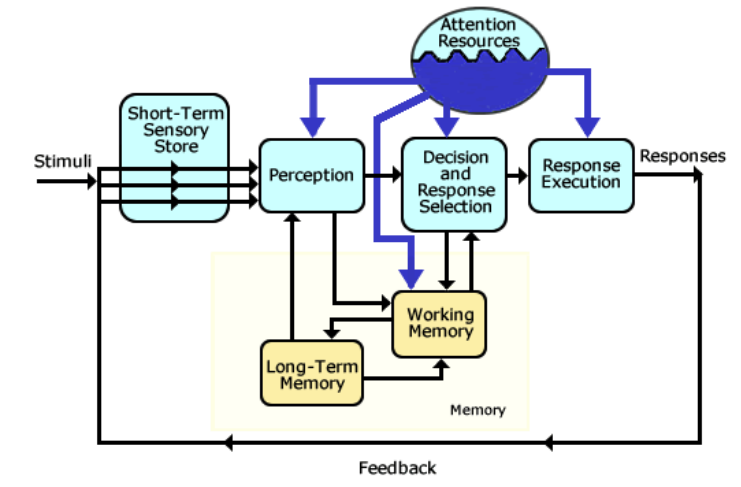
\includegraphics[width=.5\textwidth]{img/ch03_hip_overview}
	\caption{HIP -- Overview}
	\label{hip}
\end{figure} 


\subsection{Senses}:
A sense is a system that consists of a sensory cell type (or group of cell types) that respond to a specific kind of physical energy, and that correspond to a defined region (or group of regions) within the brain where the signals are received and interpreted.\\
Six external senses: sight, hearing, touch, smell, taste, balance\\
Three internal senses: thermoception, nociception (for pain), proprioception 

\subsection{Short-Term Sensory Storage (STSS)}
Sensory Memory is the retention, for brief periods of time, of the effects of sensory stimulation.\\
$\rightarrow$ Collecting information for processing, holding it briefly while initial processing is going on, filling in the blanks when stimulation is intermittent.\\
STSS does not need explicit attention, it works pre-attentive and is not part of the conscious memory. Note that STSS != short term memory.\\
Two most important types of short-term sensory memory:
\begin{itemize}
\item echoic memory (lasts $\approx 2-10s$ after stimulus) $\rightarrow$e.g. ``What did you say?''
\item iconic memory (lasts $\approx 0.5-1.0s$ after stimulus) $\rightarrow$e.g. grid of letters
\end{itemize}

\subsection{Perception}:
Human capability of information processing is limited! It is not only of interest, how much information is presented to a human, but
\begin{itemize}
\item how much information is transmitted from stimulus to response
\item capacity of the information channel
\item how rapidly information is transmitted (bandwidth)
\end{itemize}
Raw sensory data must be interpreted and given meaning. This process is called perception. It generally happens automatically (little attention needed) and fast (in contrast to cognitive processes).
\begin{itemize}
\item driven by sensory inputs $\rightarrow$bottom-up
\item driven by long-term memory $\rightarrow$top-down
\end{itemize}

\subsection{Attention}
Attention is the cognitive process of selectively concentrating on one aspect of the environment while ignoring other things. It is the crucial element for cognitive processes as
learning or task execution. Types of attention:
\begin{itemize}
\item selective attention: willingly select focus
\item focused attention: respond to external events
\item divided attention: simultaneous focusing on different events
\end{itemize}
\textbf{Allocation Model of Attention (Kahneman, 1973)}:
Limited amount of ``processing power'' at our disposal. Task execution depends on how much of our attention ``capacity'' we can spare on it.
\textbf{Controlled and Automatic Attention (Schneider and Shiffrin, 1977)}:
\begin{itemize}
\item Controlled processing makes heavy demands on attentional resources, is slow and limited in capacity, and involves consciously directing attention towards a task.
\item Automatic processing makes no demands on attentional resources, is fast, unaffected by capacity limitations, unavoidable and difficult to modify, and is not subject to conscious awareness
\end{itemize}
\textbf{Selective and Focused Attention}:
Concentration on one stimulus source needed for e.g. perception or learning (visual sampling or scanning). Being too selective is referred to as ``cognitive tunneling''.\\
Negative examples: selecting cues that stand out rather than useful ones (e.g. during a presentation/argumentation).\\
Humans have tendency to be distracted $\rightarrow$important e.g. for directing attention to warning/error messages\\
Differences in errors between selective attention and focused attention: intentional selection of the wrong source vs. unintentional external influences.\\
\textbf{Divided Attention}:
C.f. attention models. Limited attention capacity of humans, important e.g. for layout of instruments in a cockpit (see Gestalt laws). Differences in errors between focused attention and
divided attention: some of our attention is directed to stimuli we do not wish to process vs. our limit to attend to all stimuli we wish to process.\\
$\rightarrow$ Only a certain maximum of attention capacity can be divided to tasks!\\

Attention can be directed at a particular task and/or divided between a number of different tasks. Practice reduces the amount of attention required by a particular task (e.g. typing blindly on a keyboard while reading a text). Attention and awareness are closely linked.

\subsection{Vigilance}
Vigilance is an aspect of attention which refers to detecting a rare event or signal in a desert of inactivity or noise.
It means to detect signals over a long period of time which are intermittent, unpredictable, and infrequent, but it is known that they happen.\\
Examples of vigilance tasks: security inspector x-raying luggage, quality control in production\\
$\rightarrow$vigilance level (steady-state level performance)\\
$\rightarrow$vigilance decrement

\textbf{Paradigms}
\begin{itemize}
\item free-response paradigm: a target event occurs at any time, non-events are not defined; example: power plant monitor supervision
\item inspection paradigm: events occur at fairly regular intervals; some are events, most are non-targets; example: quality control (most items are ok, only some have defects)
\item successive vigilance paradigm: target stimulus has to be remembered; successive events have to be compared to the target stimulus; example: detect if a color is darker than the initial target
\item simultaneous vigilance paradigm: all events/information needed for discrimination are present at the same time; example: compare many types of garment to a standard piece of fabric
\item sensory vigilance paradigm: signals represent changes in the auditory or visual intensity; example: color changes
\item cognitive vigilance paradigm: signals represent ``information'' (symbolic or alphanumeric stimuli); example: proofreading a manuscript
\end{itemize}

\subsection{Workload and Measurement -- Signal Decision Theory}
The SDT model assumes that there are two stages of information processing in the task of detection: Sensory evidence is aggregated concerning the presence or absence of the signal. A decision is made about whether this evidence indicates a signal or not.\\
Signal detection \& neural activity: External stimuli generate neural activity. On average, there will be more neural evidence when a signal is present than when it is absent.\\

Types of noise:
\begin{itemize}
\item internal (in our brain, e.g. firing rate of neurons varies for the same stimulus)
\item external (in the data) internal response (in the observer’s brain)
\end{itemize}
The probability distributions for internal response can be different for noise and for signal! Internal response as neural activity resulting from a stimulus:
\begin{figure}[h!]
	\centering
	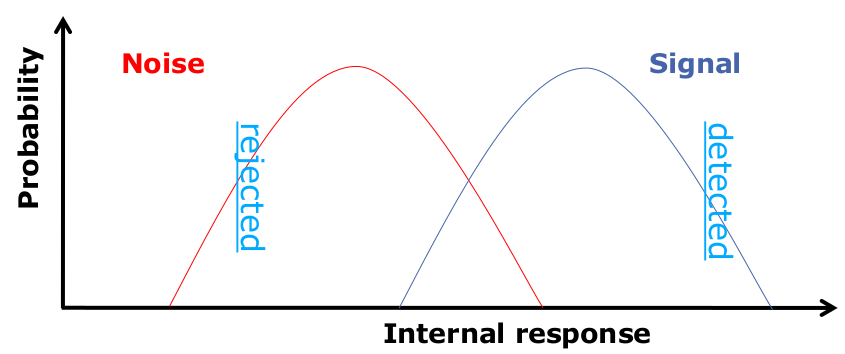
\includegraphics[width=.5\textwidth]{img/ch03_std.png}
	\caption{}
	\label{std}
\end{figure} 
\begin{figure}[h!]
	\centering
	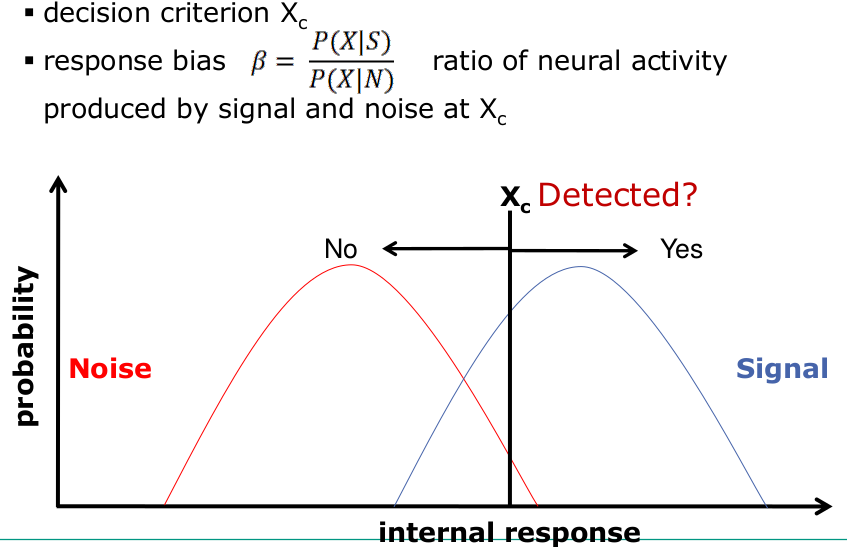
\includegraphics[width=.5\textwidth]{img/ch03_std1.png}
	\caption{}
	\label{std1}
\end{figure} 
\begin{figure}[h!]
	\centering
	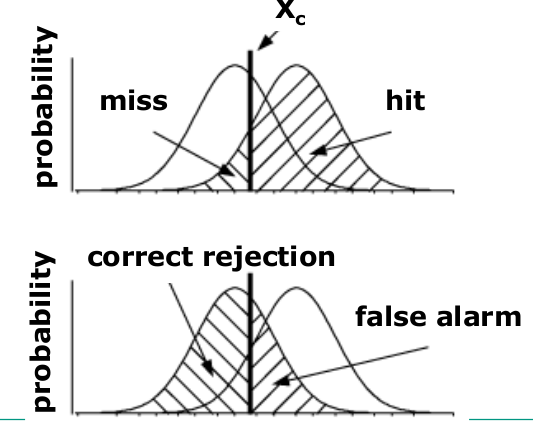
\includegraphics[width=.3\textwidth]{img/ch03_std2.png}
	\caption{signal classifications revisited: hit, miss, false alarm and correct rejection}
	\label{std2}
\end{figure} 
Optimal beta (bias) should be set where the probability of signal and noise are equal. $\beta_{opt}$ tells us where the bias should be, while $\beta$ tells
us where the bias really is. $\beta_{opt} = \frac{P(N)}{P(S)}$\\
Usually, humans adapt ``their'' beta not enough (too conservative or too risky):\\
$\rightarrow$Over-estimation of rare events\\
$\rightarrow$Under-estimation of frequent events\\
$\rightarrow$``Sluggish beta'' refers to highly focused attention processes, rare attention or sub-conscious processes underestimate rare events.\\

\textbf{Sensitivity} (d’) is the resolution of the detection mechanism. It refers to the separation of noise and signal distributions along the $X$-axis (see slide 1-9??) and corresponds to the separation of the means of the two distributions.
\begin{figure}[h!]
	\centering
	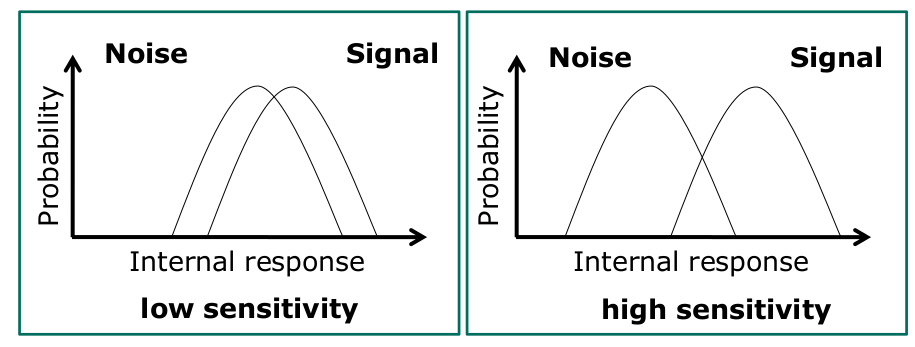
\includegraphics[width=.5\textwidth]{img/ch03_std3.png}
	\caption{Sensitivity}
	\label{std3}
\end{figure} 

\subsection{Memory}
Human memory consists of two major components: Working memory (formerly: short-term memory) and long-term memory. Memory ``processes'' include recall, recognition, chunking and rehearsal. Human memory is multi-modal! The brain makes up 2\% of a person's weight. It consumes 20\% of the body's energy, even at rest. Brain energy consumption is 10 times the rate of the rest of the body per gram of tissue. Average power consumption of a typical adult lays at 
100 Watts brain consumes 20\% (20W) of this.

\textbf{Working Memory}
\begin{itemize}
\item Memory storage for up to 30 seconds, after that short period, the contents decay or are displaced.
\item rapid access: $\approx$ 70ms access time
\item storage size: 3-4 ``chunks'' (NOT: 7+-2 elements!)
\item it is easy to overwrite the contents (intentionally and
unintentionally!)
\item can store two different types of data at the same time: visual information (visuo-spatial sketchpad) \& verbal information (articulatory loop)
\item to maintain the contents of working memory: rehearsal is needed
\item to persistently store information from working memory: move it to long-term memory
\end{itemize}
Types of WM:
\begin{itemize}
\item Verbal: Phonological Store\\
$\rightarrow$ Retrieval: Articulatory loop
$\rightarrow$ ``Programmed'' and associated by words written, spoken (the latter are simpler to remember)
\item Visual; Visuospatial Sketchpad, stored often in form of images
\item Operate in parallel, but there is only a restricted number of attention levels
\end{itemize}
\textbf{Long-Term Memory}
\begin{itemize}
\item ``unlimited'' in capacity
\item lasts from a few minutes to life time
\item slow access: 100ms seconds access time
\item multi-modal memory: smell as strong trigger to long-term memory (sound as most efficient cue for working memory)
\item three types (could be clustered otherwise, depending on psychological model): episodic – serial memory of events, procedural – knowledge of how to do things, semantic – structured memory of facts, concepts, skills
\item semantic LTM ($\rightarrow$ relationships between bits of information, inference through inheritance) derived from episodic LTM
\item Forgetting: decay (information is lost gradually, but very slowly), interference (retroactive interference: new information replaces old, proactive inhibition: old may interfere with new);  affected by emotion (can subconsciously `choose' to forget)
\end{itemize}
\begin{figure}[h!]
	\centering
	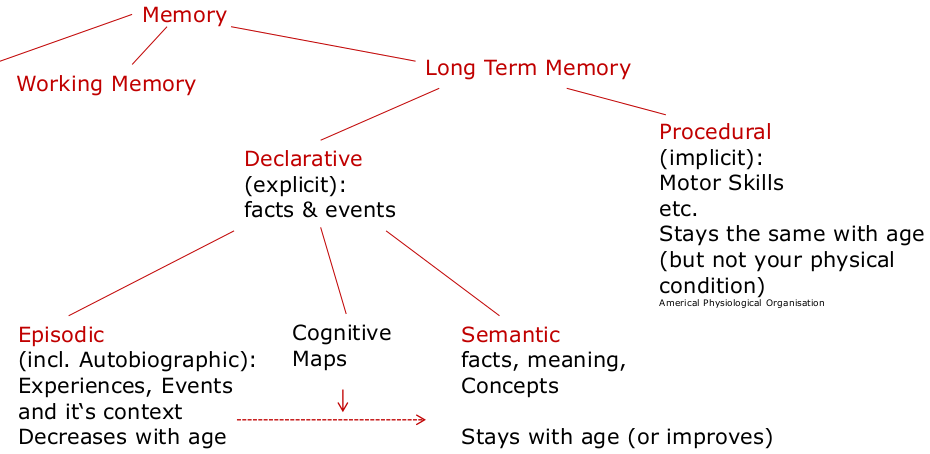
\includegraphics[width=.5\textwidth]{img/ch03_mem.png}
	\caption{}
	\label{Memory Model}
\end{figure} 
Long Term Memory Processes:
\begin{itemize}
\item Encoding is the process by which information is stored in memory.
\item Retrieval is the means by which memories are recovered from long-term storage.
\item Forgetting is the name of a number of different possible processes by which we fail to recover information.
\item recall (``Erinnerung''): active memory search to retrieve a particular piece of information
\item recognition (``Wiedererkennung''): searching the memory and deciding whether the retrieved piece of information matches a given information; recognition is generally easier and quicker than recall!
\item[$\rightarrow$] Icons often use metaphor to recall an associated object or activity\footnote{Horton‘s checklists for icons: Understandable, Familiar, Unambiguous, Memorable, Informative (concept important?), few (<20), distinct, attractive, legible (tested in all view contexts), compact (means minimal), coherent (can be separated from other icons and the background), extensible (means size scalable)}
\item rehearsal: There is no direct link from perception to LTM! The process of repeating information in working memory. This facilitates the short-term recall of information and its transfer to long-term memory. The amount stored is proportional to the number of rehearsals!
\item chunking: grouping of items into more meaningful units
\end{itemize}

\subsection{Memory Design Guidelines}\footnote{Guideline: specific and practical rules for solving problems of UI design;\\ Principles: help for analyzing and comparing design alternatives;\\
Theories and Models: describe objects and actions with consistent terminology and give a comprehensible explanation of connections}
\begin{itemize}
\item[M1:] Organize information into a small number of ``chunks''.
\item[M2:] Try to create short linear sequences of tasks.
\item[M3:] Use persistence, so do not flash important information onto the screen for brief time periods.
\item[M4:] Do not ``overwrite'' the contents of working memory by giving additional tasks to the user.
\item[M5:] Organize data fields to match user expectations or to organize user input (e.g. the automatic formatting of phone numbers)
\item[M6:] Provide reminders or warnings of the state the user has reached in an operation.
\item[M7:] Provide ongoing feedback on what is happening and/or what has just happened.
\item[M8:] The user interface should behave in consistent ways at all the times for all screens.
\item[M9:] Terminology, icons and the use of colour should be consistent between screens.
\end{itemize}

\subsection{Decision Making}
Semantic coding: without memory, there is no ``thinking'' or decision-making! After the perception of the stimulus, a response needs to be selected.\\
Automatic vs. controlled decisions:
\begin{itemize}
\item automatic($\rightarrow$ fast): little or no attention required, learned reflexes or behavior, a long-term memory procedure is executed nearly automatically in response to the stimulus
\item controlled ($\rightarrow$ slow): attention required, typically conscious of thoughts, interaction with WM and LTM systems
\end{itemize}
\subsection{Response and Feedback}
After a decision has been made, it has to be executed by complex motor movements.\\
Feedback-loop: we observe the consequences of our actions, producing closed-loop feedback $\rightarrow$ the model is circular rather than linear (\autoref{hip})!

\subsection{HIP by Numbers}
\textbf{CMN-Model} (Card, Moran \& Newell, 1983):\\
Three interacting subsystems, each with processor \& memory and described by parameters; serial \& parallel processing
\begin{enumerate}
\item Perceptual processor: receives sensory input (audio \& visual), codes info symbolically, output into audio \& visual image storage (WM buffers)
\item Cognitive processor: input from sensory buffers, can access LTM to determine response according to previously stored info, output response into WM
\item Motor processor: input response from WM, carry out response
\end{enumerate}
Subsystem interations in terms of input/output. Processing:
\begin{itemize}
\item serial action: e.g. pressing key in response to light
\item parallel perception: e.g. driving, reading signs \& hearing
\end{itemize}
\textbf{Parameters} (based on empirical data):\\
Processors have: cycle time ($\tau$)\\
Memories have: storage capacity ($\mu$), decay time of an item ($\delta$), info code type ($\kappa$, physical, acoustic, visual \& semantic)
\begin{itemize}
\item Processor cycle time: $\tau_{per} = 100ms$, $\tau_{cog} = 70ms$, $\tau_{mot} = 70ms$ $\rightarrow$ total time: $\tau_{per} + \tau_{cog} + \tau_{mot}$
\item Visual image store:  $\mu_{per} =$17 letters (visual) bzw. 5 letters (auditive), $\mu_{WM} =$3-7 chunks
\item Decay time (half-life index): $\delta_{per}=200ms$ (visual), $\delta_{per}=1500ms$ (auditive); $\delta_{WM}=7s$ (for 3 chunks), $\delta_{WM}=73s$ (for 1 chunk) 
\item Info code type: $\kappa$ = physical $\rightarrow$ physical properties of visual stimulus (e.g. intensity, color, curvature, length)
\end{itemize}
Principle of Operation -- Power Law of Practice: task time on the $n^th$ trial $T_n = T_1n^{-0.4}$ $\rightarrow$ you get faster the more times you do it, applies to skilled behaviour (perceptual \& motor) but not to knowledge acquisition\\
$\Rightarrow$ These numbers are used later for the interaction design models

\section{Perception}
\subsection{Visual Perception: Illusions and Gestalt Theory}
Visual perception is the process of extracting meaning from sensory information. It is concerned with recognition and understanding.
Vision is an easier process concerned with detecting color, shapes or edges of objects. Vision does not necessary require an understanding of the world surrounding us.\\
The Gestaltists, a group psychologists, identified a number of properties that can be regarded as innate to all humans. \\
Gestalt Laws: methods that the brain uses to simplify recognition by ordering them
\begin{enumerate}
\item Proximity: Objects that are close in space or time tend to be perceived together. This can be used e.g. for UI arrangement of buttons or information.
\item Common fate: Principle – Objects that ''move” together are seen as related
\item Prägnanz -- Law of Good Gestalt: Complex an unknown figures are automatically separated into known simple forms to make sense of them
\item Closure: Tendency to see things as complete objects even though there may be gaps in the shape of the objects. Closed figures are perceived more easily than incomplete or open figures.
\item Continuity: Tend to perceive smooth, continuous patterns instead of disjoint, interrupted patterns.
\item Similarity: Similar figures tend to be grouped together.
\item Part-whole relationships
\item Symmetry
\item Area Principle (also called the smallness principle): Objects with small area tend to be seen as the figure, not the ground.
\item Surroundedness Principle: An area that is surrounded will be seen as the figure and the area that surrounds will be seen as the ground.
\end{enumerate}
Other Principles of Perception:
\begin{itemize}
\item Stimulus Intensity: We respond first to the intensity of a stimulus and only then do we begin to process its meaning.
\item Proportion: can be used to represent logical hierarchies (e.g. font size of headings, subheadings...)
\item[$\rightarrow$] Golden Ratio: $\frac{a+b}{a}=\frac{a}{b}$The golden ratio expresses the relationship between two aspects of a form such as height to width and must equal 0.618; is seen as aesthetic
\item[$\rightarrow$] Fibonacci: A sequence of numbers in which each number is the sum of the two preceding numbers. The relationship between the numbers in the Fibonacci series is similar to the golden ratio.
\item Screen Complexity (Tullis, 1984): can be used to calculate the relative complexity, and therefore the difficulty, of a design. This measure of complexity uses information theory (Shannon \& Weaver, 1949) $C = -N \sum\limits_{n=1}^m p_n \log_2 p_n$ with 
\begin{itemize}
\item $C$ = complexity of the system in bits
\item $N$ = total number of events (widths or heights)
\item $m$ = number of event classes (number of unique widths or heights)
\item $p_n$ = probability of occurrence of the $n^{th}$ event class (based on the frequency of events within that class)
\end{itemize}
Calculating screen complexity:
\begin{enumerate}
\item Place a rectangle around every screen element
\item Count the number of elements and the number of columns (vertical alignment points)
\item Count the number of elements and the number of rows (horizontal alignment points) 
\item[$\rightarrow$] lowering these numbers reduces visual complexity (law of common fate, closure) 
\end{enumerate}
\begin{figure}[h!]
	\begin{subfigure}{.7\textwidth}
	\centering
	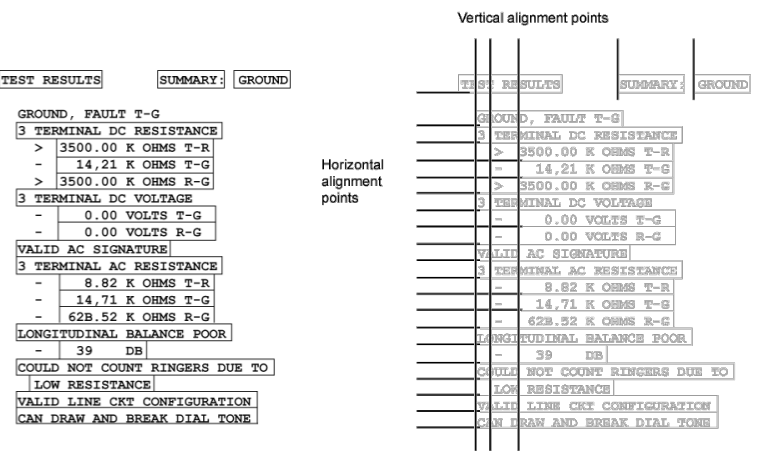
\includegraphics[width=.7\textwidth]{img/ch04_sc}
	\subcaption{Complexity Analysis}
	\end{subfigure}
	\begin{subfigure}{.5\textwidth}
	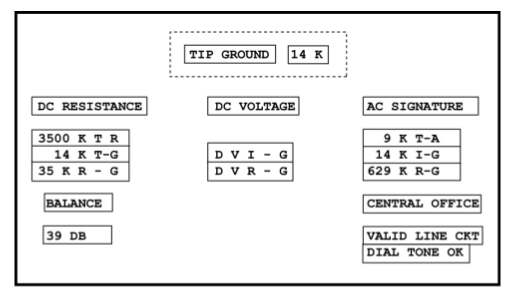
\includegraphics[width=.5\textwidth]{img/ch04_sc1}
	\centering \subcaption{Improved Interface}
	\end{subfigure}
	\caption{Example}
\end{figure}
\item[$\rightarrow$] Comber and Maltby (1997): both overly simple and overly complex screens low in usability (in terms of Effectiveness, Learnability, Attitude)
\end{itemize}
\textbf{Depth Perception}
Types of depth cues:\\
\begin{itemize}
\item Primary depth cues (relevant e.g. to immersive virtual reality systems)
\begin{itemize}
\item retinal disparity: As our eyes are approximately 7cm apart, each retina receives a slightly different image of the world. This is processed by the brain and interpreted as distance information.
\item Stereopsis: Process by which the different images of the world received by each eye are combined to produce a single three-dimensional experience.
\item Accommodation: A muscular process by which we change the shape of the lens in our eyes in order to create a sharply focused image. The information from the muscles is unconsciously used for depth information.
\item Convergence: Over distances of 2-7m we move our eyes more and more inwards to focus on an object at these distances. This process is used to provide additional depth information.
\end{itemize}
\item Secondary depth cues (more relevant e.g. to non-immersive applications such as games)
\begin{itemize}
\item Light and shade: An object with light and shadow improves the depth perception.
\item Linear perspective
\item Height in the horizontal plane
\item Motion parallax: Near objects are perceived to flash by quickly, objects further away as slower.
\item Overlap: e.g. overlapping windows in a GUI
\item Relative size: see sun + cloud
\item Texture gradient: textured surfaces appear closer
\end{itemize}
\end{itemize}
\subsection{Usability: Goals -- Principles -- Guidelines}
\begin{itemize}
\item Usability Goal -- Easy to use: most people do not want to struggle with tools are interested in completing their tasks
\item Design Principle -- Simplicity: Simple things require little effort and can often be accomplished without much thought. If interaction designs are guided by the principle of simplicity, they will be easier to use.
\item Project Guideline -- Dialog Boxes: All dialogue boxes should present only the basic functions that are most often used and that other, less used functions can be accessed using an expandable dialogue with a link for ''More Options”.
\end{itemize}
\subsection{Colors}
Additive (displays) and subtractive (printed) color mixing.\\
\textbf{Limitations}: 
\begin{itemize}
\item Blue Color is on the edge of the spectrum $\rightarrow$ Avoid using blue color for small and tiny elements.
\item The ability to distinguish color is directly related to the size of an object!
\item Shapes are identified by their edges. Edges are faster identified by lines than by colors.
\item Better color perception in the middle of the focus.
\item About 8\% of male (0.4\% of female) have deficiencies to perceive colors correctly. Most common deficiency is detection of green
\item Colors may cause problems leading to divided attention (as shown in Stroop test)
\item Colors may cause emotional response: varies depending on culture, age, sex $\rightarrow$ Industries, professional communities, corporate have their own colour connotations
\end{itemize}
\textbf{Colors for Design -- Color Coding -- Optimal Colors}
\begin{itemize}
\item For Clarification, Relation, Differentiation: e.g. Subway Maps
\item Support finding: e.g. important element in a text
\item Comprehension, Retention and Recall: e.g. Levels of danger, different measurements in a scatter plot etc.
\item Color coding can improve recall, search-and-locate tasks, decision judgements $\rightarrow$ overall performance but does not replace good structure!
\item Avoid any incompatible color combination, e.g. bright red on blue (background to foreground contrast)
\item Color presentation and perception change with medium and display technology; light in the workspace may influence color perception
\item Thorell \& Smith: red, blue, green and yellow are most beneficial in learning environments
\item Using a color code: Max 4 main colors, each having max 4 variants; structure the content and identify the content that should be supported with a color
\end{itemize}
\subsection{Hearing}
\textbf{Loudness} (dB): dB is a logarithmic scale; Frequency range of hearing 20Hz-20kHz\\
\textbf{Four Stages of Auditory Perception}
\begin{itemize}
\item Transduction: Translation of sound vibrations into neural impulses
\item Auditory grouping: Segregation into separate streams + Integration of sound in coherent streams (based on similar harmonic, frequency, location etc.)
\item Scene Analysis
\item Interpretation
\end{itemize}
\textbf{Audio User Interfaces}: Vision and Hearing go together, but audio can give impression from area that are beyond vision (audio can tell your eyes where to look). However, people become habituated to continuous sounds and ignore important sound based information. Continuous sounds requires resources from the human, even if it is a continuous sound, leading to additional stress. Audio can be perceived faster than visual cues. Audio is transitory! Vision is often not!\\
\textbf{(Non-)Speech}: We can speak faster than we can write, but spoken interaction contains more redundancy in terms of content. Speech requires knowledge of language. We can read faster than we can listen. It is often therefore more efficient to read than to listen. Listening is a liner task. Reading can jump! Auditory feedback can be non-speech. Beyond simple forms, sounds must be learned or familiar. They can be annoying and ambiguous and there are not so many expressions possible.\\
$\rightarrow$ Use of Sound:
\begin{itemize}
\item Redundant Coding: E.g. the ``click'' sound when pressing a GUI button\\
$\rightarrow$ redundant coding aids recalling an interaction by giving additional association\\
$\rightarrow$ can increase efficiency for tasks, as experts can react faster (on sound only)\\
$\rightarrow$ people with deficits (e.g. color blindness) may benefit from redundant coding\\
$\rightarrow$ Can be used for emotion (e.g. the ``miauw'' sound of my camera)\\
$\rightarrow$ Most important: Positive / Negative-Feedback\\
\item Speech applications
\end{itemize}
Use Case: Nomadic Radio	

\section{Design Analysis}
\subsection{Foundation Laws}
\textbf{Physical Models -- Fitts' Law}:\\
Physical models can predict efficiency based on the physical aspects of a design. They calculate the time it takes to perform actions such as targeting a screen object and clicking on it.
Fitts' law can be used to determine the size and location of a screen object. It states that the time it takes to hit a target is a function of the size of the target and the distance to that target:

\begin{itemize}
\item Index of Difficulty (ID): Quantifies the difficulty of a (motor pointing) task based on width and distance
\begin{align*}
ID = \log_2(A / W+1)
\end{align*}
$A$=amplitude, $W$=width
\item Movement Time (MT): Quantifies the time it takes to complete a task based on the difficulty of the task (ID) and two empirically derived coefficients that are sensitive to the specific experimental conditions\\
\begin{align*}
MT = a + b \log_2(A / W+1) = a + b ID
\end{align*}(assuming linear movement speed).\footnote{Original form: $MT = a + b \log_2(2A / W)$}
$a \left[sec\right], b\left[sec/bits\right]$ constants dependent on the input device\\
$\rightarrow$ Fitts' law (1954) predicts that the time to acquire a target is in logarithmic relation the target size.\\
\begin{figure}[h!]
	\centering
	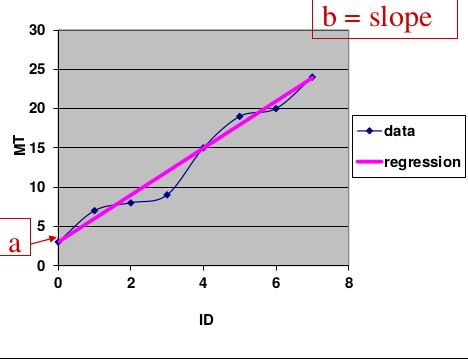
\includegraphics[width=.5\textwidth]{img/ch05_fitt.png}
	\caption{Linear Regression Model}
	\label{fitt}
\end{figure} 
\item Index of Performance (IP), also called throughput (TP): Based on the relationship between the time it takes to perform a task and the relative difficulty of the task
\end{itemize}
In practice $A$ corresponds to the distance from starting position, $W$ to the size of target along the line of motion. Common parameter values (e.g. for a mouse) are $a=50ms, b=150ms/bit$.
\begin{figure}[h!]
	\centering
	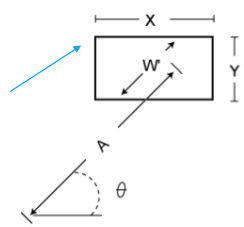
\includegraphics[width=.3\textwidth]{img/ch05_fitt1.png}
	\caption{Fitts' law in practice.}
	\label{fitt1}
\end{figure}
Fitt's Law is a predictive model of time to point at an object. Implications for interaction design in GUIs:
\begin{itemize}
\item Doubling the distance increases time but does not double it.
\item Increasing target size enables more rapid pointing.
\item MT for ``gross-movement tasks'': Formula from above, where $a$= time to start and stop in seconds for a device and $b$ = inherent speed of the device (e.g. a mouse)
\item Movement Time (MT) for ``precision pointing tasks'': $PPMT = a + b \log_2 (A/W + 1) + c log_2 (d/W)$, where $c$ = added constant, dependent on the user's context and $d$ = distance between hand location and spot where the user first touched the screen
\item GUIs with a Mouse Interface: 
\begin{itemize}
\item Overly elongated objects hold no advantage (W/H ratios of 3 and higher)
\item Objects should be elongated along the most common trajectory path (widgets normally approached from the side should use W, those approached from the bottom or top should use H).
\item Objects should not be offset from the screen edge
\item Fitts law does not address touch specific problems, e.g. fat finger
\end{itemize}
\item Fitts' Law is not 1:1 applicable to touch interfaces:
\begin{itemize}
\item Fat finger problem
\item Fingers are not moving directly from target to target but make a 3D movement
\item Fingers may directly reach target or need to be stretched or bended or a user may be even forced to change to 2-handed input
\item Screen size and hand size have a major impact on performance
\end{itemize}
\end{itemize} 
\textbf{Modelling Structure -- Hick's Law}:\\
Hick's Law states that the time $T$ needed to make a decision (e.g. a selection) is proportional to the log number of alternatives given.
\begin{align*}
T = b \cdot H
\end{align*}
where $H$ is the information-theoretic entropy of a decision:
\begin{align*}
H = 
\begin{cases}
\log_2(n+1), & n = \text{ alternatives of equal probability}\\
\sum p_i \log_2(\frac{1}{p_i + 1}), & p_i = \text{ probability of alternative }i
\end{cases}
\end{align*}
Note: Hick's Law does not apply if it requires linear search (e.g. a randomly ordered list of commands in a menu). It applies if the user can search by subdivision.\\
The total decision time in practice amounts to 
\begin{align*}
T = a + b \log_2(n+1)
\end{align*}
where $n$ is the number of choices. The coefficients are empirically determined from experimental design. Raskin (2000) suggests that $a= 50 ms$ and $b=150 ms/bit$ are sufficient place holders for ``back-of-the-envelope'' approximations.

\textbf{Power Law of Practice}:\\
Users get better every time they use a system. Neglecting disturbance and decay effects
\begin{align*}
Time = B\cdot N^{-\alpha}
\end{align*}
where $N$ = Trial Number, $B, \alpha$ = constants

\subsection{Applied Design Guidelines \& Principles: Mental Models -- Mapping -- Affordances}
\textbf{Mental Models}: \\
People use a mental model to have a basic understanding of what is going on. The mental model is often unsharp, e.g. you know your car speeds up when pressing the gas pedal, but the concept behind is unsharp. Unsharp models might be sufficient, but in certain situations they might not be enough to explain the system. Interaction that is both predictive and explanatory can be understood with the concept of mental models. Mental models are
\begin{itemize}
\item Unscientific: they are based on guesswork
\item Partial: They do not describe the whole system
\item Unstable: They evolve an adapt to context and experience
\item Inconsistent: Some parts of the model may be incompatible with other parts of the system
\item Personal: They are specific to individuals
\end{itemize}
However, they can be used to foster understanding and building a correct model and thus increase usability. E.g. Error Avoidance Design Guidelines exploit natural mappings between intentions and possible actions, between actions and their effects on the system state and what is perceivable, as well as between the system state and the needs, intentions and expectations of the user.\\

\textbf{Principles of Good Design (Don Norman)}:\\
An interface should include good mappings that show the relationship between stages. There should be a clear correlation between control element and action. A ``good'' mapping should be understandable, consistent, recognizable or quickly learnable and natural (consistent to the user's knowledge, world and domain knowledge). For example for cooking plates it would be helpful to arrange the buttons corresponding to the plates exactly like the plates themselves.\\ \\

\textbf{Constraints} lead humans to build correct mental models. They guide the user to the next appropriate action or decision and also minimize the chance to make errors.
\begin{itemize}
\item physical constraints (dial vs. button)
\item semantic constraints (assumption that create something meaningful)
\item cultural constraints (borders provided by cultural conventions, e.g. traffic signs, colours, ..)
\item logical constraints (restrictions due to reasoning)
\end{itemize}
It is good (for safety) to add some redundancy, as constraints can only work at their own level (e.g. having plugs color- and shape-coded in safety-critical situation).\\

\textbf{Affordances (Gibson)}:\\
To build a mental concept of a system we need to interpret symbols and components. This can be seen as the functionality of the device and what we actually want to do\\
$\rightarrow$ Semantic and Articulator Distance\\
Don Norman developed this concept further picking up the idea of affordances. It refers to the perceived and actual properties of an (everyday) object, which have to be matched:\\
-- Make usable properties visible\\
-- Use natural associations\\
-- Give Feedback\\
Objects and environments imply their usage through Gestalt, e.g. door handle animates to press, cup to drink $\rightarrow$ Partially learned!\\
\textbf{Normans Evaluation/Execution Action Cycle}:
\begin{figure}[h!]
	\centering
	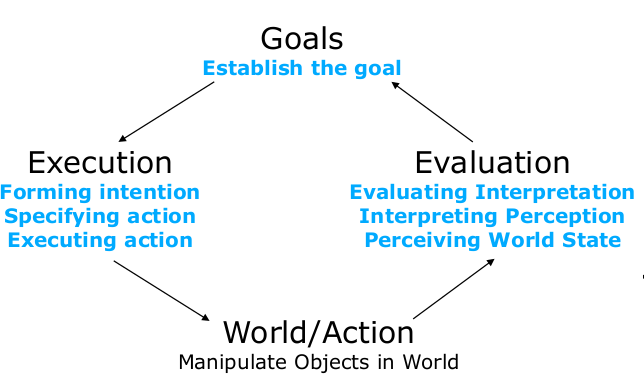
\includegraphics[width=.4\textwidth]{img/ch05_cycle1.png}
	\caption{Evaluation/Execution Action Cycle}
	\label{cy}
\end{figure}
\begin{itemize}
\item Gulf of execution: Mismatch between the user's intentions and the allowable actions. Problems:
\begin{itemize}
\item Forming intention $\rightarrow$ Insufficient knowledge of concept
\item Specifying action $\rightarrow$ Insufficient knowledge of usage
\item Executing action $\rightarrow$ Difficult access to function
\end{itemize}
The difference between the intentions and the allowable actions is the Gulf of Execution. How directly can the actions be accomplished? Do the actions that can be taken in the system match the actions intended by the person?\\
$\rightarrow$ Good design minimizes the Gulf of Execution
\item Gulf of evaluation: Mismatch between the system's representation and the users' expectations. Problems:
\begin{itemize}
\item Evaluating Interpretation $\rightarrow$  Comparing goal and state
\item Interpreting Perception $\rightarrow$ Interpretation of state
\item Perceiving World State $\rightarrow$ perception of State
\end{itemize}
You may check how easy you are able to determine the function, determine what actions are possible, determine mapping from intention to physical movement, perform the action, determine whether the system in the desired state, determine mapping from system state to interpretation and determine what state the system is in. The Gulf of Evaluation reflects the amount of effort needed to interpret the state of the system and how well this can be compared to the intentions. Is the information about state of the system easily accessible? Is it represented to ease matching with intensions?\\
$\rightarrow$ Good design minimizes the Gulf of Evaluation
\end{itemize}

Example: The user wants a document written on the system in paper (the goal).\\
Gulf of Execution: What actions are permitted by the system to achieve this goal?\\
Gulf of Evaluation: Is the process observable? Are intermediate steps visible?\\
Implications on design:
\begin{itemize}
\item Principles of good design (Norman):
\begin{itemize}
\item Stage and action alternatives should be always visible
\item Good conceptual model with a consistent system image
\item Interface should include good mappings that show the relationship between stages
\item Continuous feedback to the user
\end{itemize}
\item Critical points/failures:
\begin{itemize}
\item Inadequate goal formed by the user
\item User does not find the correct interface / interaction object
\item User many not be able to specify / execute the desired action
\item Inappropriate / mismatching feedback
\end{itemize}
\end{itemize}

\subsection{Task Analysis}
A \textbf{goal} is a state of the application domain that a work system wishes to achieve. Goals are specified at particular levels of abstraction. \\
A \textbf{task} is a goal together with some ordered set of actions. Or more elaborated:
A task is a structured set of activities required, used or believed to be necessary by an agent to achieve a goal using a particular technology. A task will often consist of subtasks where a subtask is a task at a more detailed level of abstraction. The structure of an activity may include selecting between alternative actions, performing some actions a number of times and sequencing of actions.\\
An action is a task which has no problem solving associated with it and which does not include any control structure. Actions and task will be different for different people.
\textbf{Task analysis} is the study of how work is achieved by tasks. It is about understanding people and how they carry out their work (part of human-centred design):
\begin{itemize}
\item identify a set of methods people use to carry out their work
\item identify if they reach the goal
\item calculate how long it takes to reach the goal
\end{itemize}
Two main categories of task analysis methods concerned with the logic of tasks (sequence of steps to achieve a goal) and the cognitive\footnote{Cognition: thinking, solving problems, learning, memory $\rightarrow$ HIP!\\ Representations of things that people are assumed to have in their heads $\rightarrow$ mental models} aspects (understanding which cognitive processes the work system will have to undertake to achieve a goal).\\
Different Task Analysis methods can be sorted into four \textbf{dimensions}: notation, usability for communication, usability for modelling tasks, adaptability to new types of systems/aims/requirements. Task analysis is an integral part of System Development and undertaken several times, during analysis (independent from technology, understanding the ``essentials'', current way of doing things), design (cognitive load minimization) and evaluation (dependent on technology, degree of achievement of work).\\ \\
In the following, two models will be discussed: Hierarchical Task Analysis (HTA), concerned with the logic of the task, and Goal-based Task Analysis (GOMS), concerned with the cognitive analysis of the task. Both models rely on Cognitive System models (see previous chapters).\\ \\ 
\textbf{Hierarchical Task Analysis (HTA)}: 
Graphical representation of a task structure in structure chart notation: sequence of tasks, subtasks and actions as hierarchy, actions can be repeated (iteration), alternative actions possible (selection), annotations to indicate plans (optional). This is not trivial: acquisition of task and subtask descriptions, hierarchical modelling, iterative process.
\begin{figure}[h!]
	\centering
	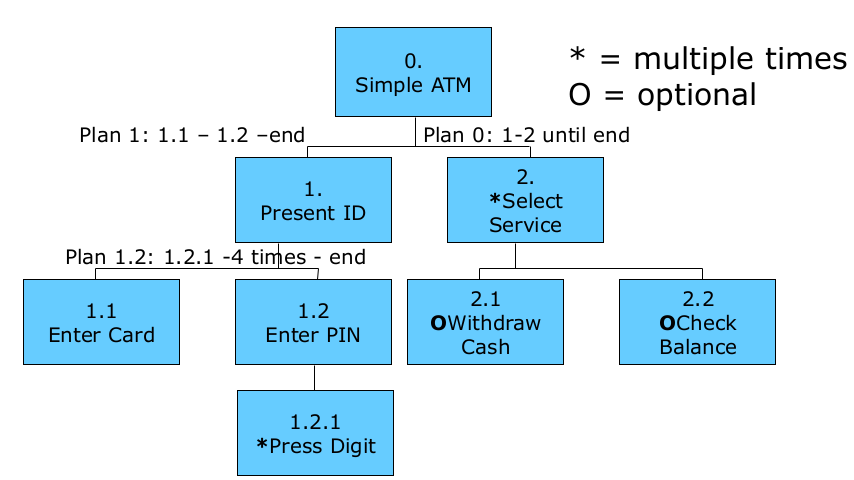
\includegraphics[width=.5\textwidth]{img/ch05_hta.png}
	\caption{HTA -- Example}
	\label{hta}
\end{figure}

\textbf{Goal-based Task Analysis -- GOMS}: Goals, Operators, Methods, Selection Rules\\
An application of Human Information Processing and Task Analysis/Decomposition focusing on Cognitive Load Analysis. Introduced by Card, Moran \& Newell (1983) they feature an explicit task structure:
\begin{itemize}
\item Hierarchy of goals and sub-goals
\item Procedure: define goals and refine them
\item Outcome are several sheets of GOMS descriptions, starting with the topmost description
\item Methods in the topmost description are subsequently refined in the ``lower'' GOMS descriptions
\end{itemize}
CNM-GOMS -- Engineering model of user interaction:
\begin{itemize}
\item Goals -- user's intentions (tasks): e.g. write a text, something the user perceives as a task
\item Operators -- actions to complete task: Basic, low level action to perform or basic mental state; cognitive, perceptual \& motor (HIP); e.g. press X, read dialog; time of activity can be given
\item Methods (Subgoals) -- sequences of actions (operators): may be multiple methods for accomplishing same goal, e.g. shortcut key or menu selection
\item Selections -- rules for choosing appropriate method: method predicted based on context; selection rules are separately described
\end{itemize}
CPM-GOMS represent Cognitive, Perceptual, Motor operators. It uses Program Evaluation Review Technique (PERT) charts which map task durations using the critical path method (CPM). It is based directly on the Model Human Processor which assumes that perceptual, cognitive, and motor processors function in parallel.
\begin{figure}[h!]
	\centering
	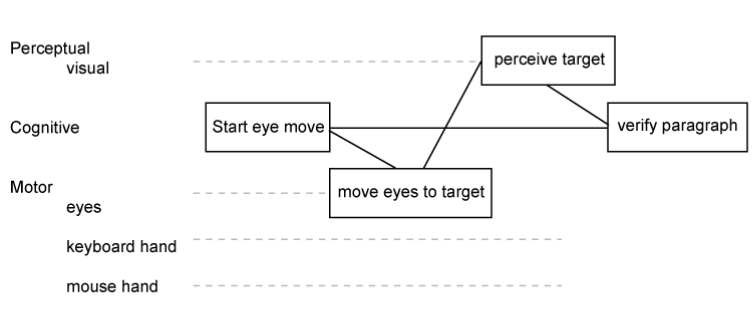
\includegraphics[width=.5\textwidth]{img/ch05_pert.png}
	\caption{PERT chart -- Example}
	\label{pert}
\end{figure}

\textbf{Keystroke Level Model (KLM)}: The KLM is a practical design tool that can capture and calculate the physical actions a user will have to carry out to complete specific tasks. It can be used to determine the most efficient method and its suitability for specific contexts. 
\begin{itemize}
\item Given:
\begin{itemize}
\item A task (possibly involving several subtasks)
\item The command language of a system
\item The motor skill parameter of the user
\item The response time parameters
\end{itemize}
\item Predict: The time an expert user will take to execute the task using the system, provided that he or she uses the method without error.
\end{itemize}
The KLM is comprised of Operators, Encoding methods, and Heuristics for the placement of mental (M) operators. Operators include \textit{Press a key or button} (K), \textit{Point with mouse} (P), \textit{Home hands to keyboard or peripheral device} (H), \textit{Draw line segments} (D), \textit{Mental preparation} (M), \textit{System response} (R)

\section{Interaction Design}
\subsection{Scenario-Based Design}
Scenarios are a foundation for the design of interactive systems. Scenario ``engineering'' involves requirements work, prototyping, envisionment, evaluation, conceptual design and physical design.

\begin{figure}[h!]
	\centering
	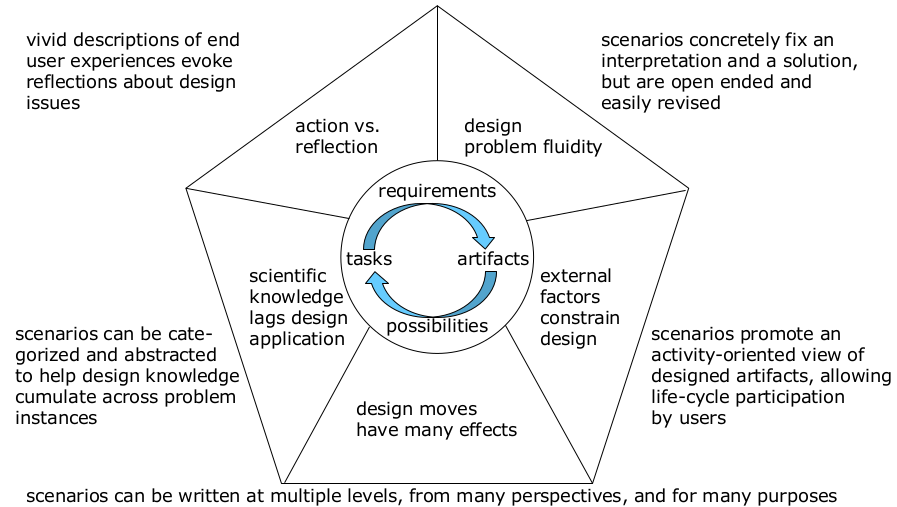
\includegraphics[width=.8\textwidth]{img/ch06_scene.png}
	\caption{Challenges and Approaches in Scenario-based Design}
	\label{scen}
\end{figure}
\textbf{Design rationale}: making the reasons for design decisions explicit. Methods for capturing and representing design rationale:\\
IBIS – issues, positions, arguments and relations
QOC – questions, options and criteria (graphical links)\\

\begin{figure}[h!]
	\centering
	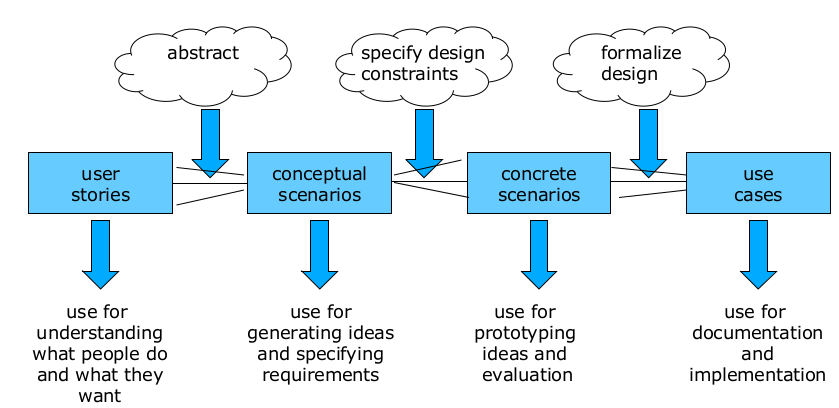
\includegraphics[width=.8\textwidth]{img/ch06_scene1.png}
	\caption{Scenarios in the Design Process}
	\label{scen1}
\end{figure}

\textbf{User Stories}: reveal ideas, anecdotes, knowledge of people, real-world experiences, activities and context. They are used to identify the problem, the stakeholders and their constraints.\\

\textbf{Conceptual Scenarios}: more abstract than user stories, derived by combining several user stories. The are used for generation of ideas and understanding requirements but do not include technology and do not specify how functions are provided.\\

\textbf{Concrete Scenarios}: derived and generated by conceptual scenarios; each conceptual scenario may generate many concrete scenarios. They suggest a particular user interface design and helü allocating functions between devices and people. They form a good start for prototyping and evaluation. \\

\textbf{Use Cases}: may result from many concrete scenarios and describe the interaction between devices and people. They abstract from concrete scenarios. Each use case covers many slight variations. Allocation of tasks and functions is needed for a use case. The sum of all use cases specifies the system design. Use cases may consist of diagrams, pseudo code, etc.

\begin{figure}[h!]
	\centering
	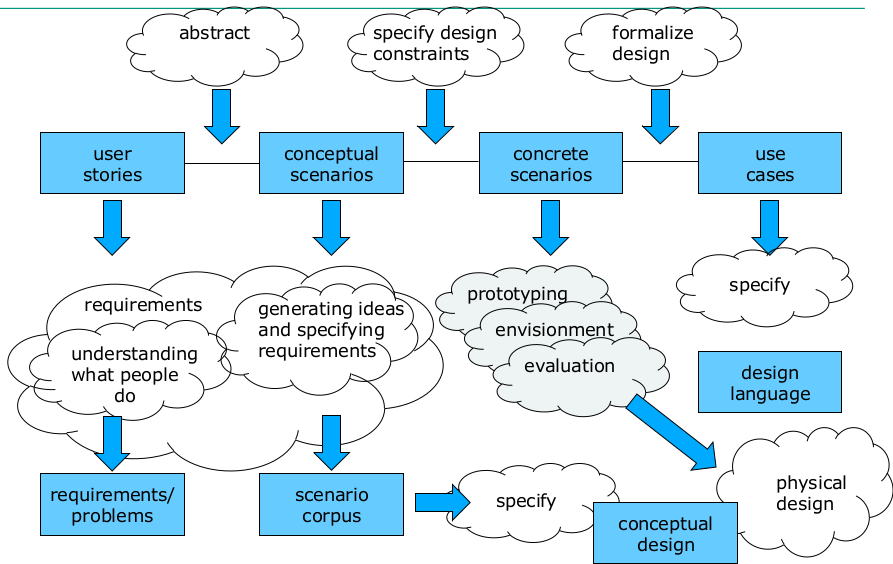
\includegraphics[width=.8\textwidth]{img/ch06_scene2.png}
	\caption{Overall Scenario-Based Design}
	\label{scen2}
\end{figure}

\textbf{Requirements and Problems}: By analysis and abstractions, difficulties become visible. In general these steps allow designers to collect experience in the formative process, in which requirements (desirable qualities of the system) can be derived. Prioritization is necessary since not all properties will be realizable.\\

\textbf{Scenario Corpus}: One wants to create a representative set of scenarios that cover a wide range of user stories. Some may be more specific, some may be more general but one takes a high-level, abstract view of the most activities in order to uncover the dimensions of the systems and the involved domains. If you don't do this, the outcome is most likely determined by technical features rather than by user requirements.\\

\textbf{Conceptual Model/Design}: An object or data model includes scenario and analysis of scenarios and describes the main objects, attributes and relationships among them. It ensures an accurate mental model of the interactive system. Here an analysis of cognitive processes, e.g. cognitive load, conceptualization is required. For example the desktop is a metaphor (mental model) for your desk.\\ 

\textbf{Design Language}: A standard set of patterns for interaction. General Design Language Concepts may be in place before concrete design application (e.g. Company Design Guidelines). Interaction patterns include physical attributes, conceptual actions and objects, key elements of design as well as principles and rules. Common language reduces the number of elements for the involved designers.

\subsection{Requirements}
Requirement analysis means understanding what people do, what people might want to do, problems with existing systems, and how people do what they do. The goal is to create ``better'' interactive systems for people. According to Robertson and Robertson (1999) a requirement is ``... something the product must do or a quality that the product must have''. Requirement work is the transformation of observation and information . It requires iterations on analysis, design, and evaluation and results in a requirements specification (formal and precise documentation of the requirements). User stories are a good start for user requirement analysis. The design process helps identifying requirements. Requirement Analysis work is very similar to software engineering! Two types:
\begin{itemize}
\item functional requirements: specify what the system must do; e.g. phone function button must be accessible while connected to the internet
\item non-functional requirements: specify what qualities the system must have, concerned with how the functionality operates; e.g. an elderly person must be able to use the phone
\end{itemize} 
For both requirement types, the technology is not yet specified, i.e. there is no specification of the implementation how-to, only usage how-to!\\
Not all requirements have equal impact on the interactive systems. Since resources are limited one needs prioritization and good balance.\\
MoSoCoW rules for prioritizing requirements:
\begin{itemize}
\item \textbf{m}ust have: fundamental requirements without which the system will be unworkable and useless, effectively the minimum usable set
\item \textbf{s}hould have: would be essential if more time were available, but the system will be useful and usable without them
\item \textbf{c}ould have: of lesser importance, therefore can more easily left out of the current development
\item \textbf{w}ant to have: will not have this time round, can wait till a later development
\end{itemize}
One may use a requirement template for functional and non-functional requirements, for project (time, man power) and design (technology) constaints:

\begin{figure}[h!]
	\centering
	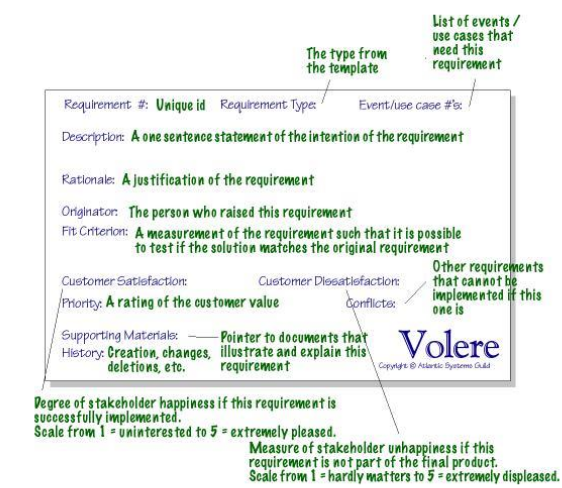
\includegraphics[width=.8\textwidth]{img/ch06_req.png}
	\caption{Using a requirement template.}
	\label{req}
\end{figure}
One can define four requirements activities, which all have the same goal:
\begin{itemize}
\item requirements gathering, which suggests requirements are lying around waiting to be picked up / explored with little interaction between designer and user. Cons: unstructured
\item requirements generation, which suggests a more creative designer activity, but tends to de-emphasize links to users' current practice.
Pros: creative. Cons: not user centered
\item requirements elicitation, suggests some user-designer interaction. Pros: user-designer collaboration. Cons: May stuck to user's creativity
\item requirements engineering, used in software engineering, suggests a very formal approach. Pros: goal oriented. Cons: formalizing to early, kills creativity
\end{itemize}
There are numerous techniques for requirements elicitation/gathering: interviews, observations, documentation (e.g. video-taping), focus groups, workshops.. (c.f. Chapter Observation). No matter which techniques are used: requirements elicitation is a user-centered activity!\\
Interviews, questionnaires and observation will identify artifacts used during the task. Most tasks require artifacts to complete. Artifacts provide additional insight in the task. Examples are documents, forms, printouts, tools..

\subsection{Envisionment}
Envisionment is concerned with making ideas visible by externalizing thoughts. The goal is to represent design work to the designers and stakeholders using stories and scenarios, presentations, sketches, formal models, software and hardware prototypes, cardboard models, mockups, ...This is fundamental to user-centered design and enables designers to see things from other people's perspective and to communicate ideas to people. It serves for generation, communication and evaluation of ideas but not all representations are suitable for all setups!\\
Exploring design concepts:
\begin{itemize}
\item how do you do it? $\rightarrow$ how do we affect the world (manipulate, sit, etc.); examples: handles (continuous) vs. buttons (discrete)
\item how do you feel? $\rightarrow$ how does the user make sense of the world, sensory qualities that shape media; satisfaction, affect, enjoyment, engagement, involvement
\begin{itemize}
\item hot media (photo): exact, authoritative, extend a single sense
\item cool media (cartoon): fuzzy and incomplete
\end{itemize}
\item how do you know? $\rightarrow$ how do people learn and plan; how designers want users to think; example: paths vs. maps (step by step vs. understanding alternatives)
\end{itemize}
\textbf{Sketches}: sketching (quickly drawing ideas and thoughts) is an important ability of a designer and used for exploration and discussion. Many ideas have been sketched out on ``the back of an envelope'' or on a napkin. Shneiderman's principle for sketches: ``overview first, zoom and filter, then details on demand'' (similar for Web-Site design!)\\
\textbf{Snapshots}: show key moments in an interaction, often refined sketches; exploring the impact of a certain style or design snapshots by sketches, storyboards or using software (e.g. Macromedia Flash, HTML, ...)\\
\textbf{Storyboards}: Technique from film making. Cartoon-like structure presenting key moments from the interactive experience: This allows people to get an idea of the flow and is an economical way to present design (6-8 scenes on one paper). There are three main types of storyboards:
\begin{itemize}
\item traditional storyboarding: as in filmmaking; scenes with notes to overcome static nature of scenes on paper; annotations of interactive behavior; good for non-multimedia user interfaces
\item scored storyboards: good for applications with motion graphics; annotation and notes about the type, colors, images, sounds
\item text-only storyboards: used for applications with complex sequences; specifies what images appear, what text comes with them, and any additional media, ...
\end{itemize}
\textbf{Mood boards} gather visual stimuli that capture something about the feeling of the design. They are widely used in advertising and interior design and may feature photographs, colors, textures, shapes, headlines from newspapers or magazines, quotations from people, pieces of fabric, ...\\
\textbf{Cultural probes} (Gaver, 1999) allow involvement and creativity and are about getting to know your target group. You prepare a set of common items (introduction how to use and what to do with the material, e.g. booklet, maps, postcards, ...; suitable prototypes). You give the items to the participants and let them use it over a certain period of time. Not all items might be used as envisioned!\\
\textbf{Navigation Maps}: Navigation is a key feature for many (complex) systems. Find out, how the user moves through the site or applications focussing on how users will experience the site. This is used to uncover functional complexity of the system and to reduce recognized complexity by better grouping navigational elements. Each page in the site or location in the application is represented with a box or heading; each page should ``flow'' from there. Navigation maps can be redrawn many times during the project lifecycle – poor navigation is a main reason to turn off customers e.g. from a website.\\
\textbf{Scenarios in Envisionment}: Scenarios, in their most concrete form, can be used to envision or evaluate specific interactions.\\
Concrete scenario $\rightarrow$  prototyping $\rightarrow$  envisonment scenarios in the figure\\
The aim is to complement scenarios with some of the more visual envisioning techniques. Scenarios in envisionment should include real data and materials to allow direct involvement and you should think hard about underlying assumptions. You should also include good characterizations and develop a good number of personas. This allows ``talking'' about the characters. Also provide rich contextual background grounding in real life forces to think about practicality and acceptability. It is impossible to write scenarios for all variations and users, but the produced scenarios should cover interactions which are typical for a number of similar use situations, important design issues which are particularly important for the focus of the project, areas where requirements are unclear, and any aspects which are safety-critical. Scenarios should be structured (e.g. title, activities, rationale). When writing, thinking about or using scenarios, issues will arise about the design space. Only when people ``see'' a concrete representation, they are able to comment meaningfully. This is achieved by e.g. notes on the storyboards, or end notes to the scenario. Often, requirements will have to be changed. You should list positive and negative features for a concrete design (capturing rationale). Scenarios are effective to bring open issues to the surface.\\
\textbf{An Outline Envisionment Process}:
\begin{itemize}
\item[1)] Review the requirements and conceptual scenarios
\item[2a)] Develop representations of the design ideas. These should include: concrete scenarios, storyboards, snapshots and sketches, ..
\item[2b)] Alternatives: If your product is a new one, experiment with different metaphors and design concepts through your representations
\item[2c)] Users: Your intended users should be involved in exploring design ideas throughout wherever possible
\item[3)] Decisions: Resources permitting, explore and document detailed design decisions using a method such as Questions, Options, Criteria (QOC)
\item[4)] Reconsider requirements in the light of the developing design, and carry out supplementary analysis where gaps in your background information have been uncovered.
\end{itemize}
\subsection{Prototyping}
Prototyping is an effective way for communicating ideas and design and complements/precedes techniques for envisionment. It is important to select the appropriate techniques. There are different levels of prototypes. Prototyping allows for participatory designs. Prototypes are a concrete but partial representation or implementation of a system. So far, screen sketches where discussed. These are, however, not interactive. Prototyping is a participatory design activity.
You could either have deep/vertical prototypes or shallow/horizontal prototypes.\\
\textbf{High Fidelity Prototypes} are  similar in look and feel to the anticipated final system. They are produced in the software that will be used for implementation or using a ``simulation'' package (e.g. using graphical toolkit: Flash, etc.) and useful for a detailed evaluation of the main design elements (content, visuals, interactivity, functionality and media). Hi-fi prototypes are also used in crucial stages of the project, e.g. client acceptance tests. They are used when the ideas, requirements and features of the system become stable. However, people might believe that the final system will exactly like the prototype! Also, a hi-fi prototype suggests that the system can be implemented/made to work! Hi-fi prototypes are costly!\\
\textbf{Low Fidelity Prototypes} are more focused on the underlying ideas, such as content, form and structure, key functionality requirements and navigational structure. They are designed to be produced quickly and thrown away after use and capture very early design thinking and should aid, not hinder, the process of generating and evaluating many possible design solutions. They often come in the form of paper prototypes (printout, paper, pen, post-its), series of screen shots. Paper prototypes are often an ideal means of prototyping interactive, screen-based systems!
Practical issues with designing paper prototypes are:
\begin{itemize}
\item robustness: can be handled by many ``users'' without breaking -- unlike a ``soldered together piece of electronics''...
\item scope: focus on broad issues and key elements; too detailed is hard to understand
\item instructions: trade-off between adding enough detail to allow the user alone to explore and between adding too much detail (so the designer needs to walk the user through)
\item flexibility: have adjustable parts (e.g. lay over other printouts e.g. on a menu, text box, ...) for visualizing interactive parts
\end{itemize}
Lo-fi prototypes usually do not ``work'' -- the designer is needed to play the computer (Wizard of Oz). Videotaping the ``interaction'' if there is much feedback. User guidance to help people access the prototype, e.g. ``setting the scene'' for a new UI for a web shop: ``You are interested in buying the shirt shown on this screen but want to know more about the material – show me what you would do now.'' Alternatively, if the system is too fragile to be exposed to users, the designers might act under the user's guidance. Much cheaper than Hi-fi, much cheaper than re-design!\\
\textbf{Trade Offs}: LoFi or HiFi Prototypes? What and how to prototype? $\rightarrow$ think in terms of PACT. Who is the prototype aimed at? What is the designer trying to achieve with the prototype? What stage of the project are things at and what is the context for use of the prototype? What technologies are appropriate?\\
According to Rosson and Carrol (2002) High-quality graphics and animation can be used to create convincing and exciting prototypes but may also lead to premature commitment to some design decision? Detailed special-purpose prototypes help to answer specific questions about a design, but building a meaningful prototype for each issue is expensive. Realistic prototypes increase the validity of user test data, but may postpone testing, or require construction of throw-away prototypes. Iterative refinement of an implementation enables continual testing and feedback, but may discourage consideration of radical transformations. Test users just get tired/used to the system.\\
Prototyping is necessary during the whole design process, but seldom done. Prototyping is much cheaper / leads to faster solution than re-implementation or project failure. ``requirements animation'': illustrating requirements by use of prototypes. Rapid prototyping for exploring the design space. Throw-away prototypes as part of the rapid prototyping activity to test/verify assumptions, but: ``You will throw away your first few designs, so you might as well plan to throw them away in the first place''.\\
\textbf{Prototype Tools}: 
\begin{itemize}
\item for requirements animation might include: PowerPoint, paper (and paper overlays), Visual Basic
\item for throw away/rapid prototyping: Adobe Flash, Web Tools
\item for incremental/evolutionary prototyping: development environment, object-oriented languages
\item for physical user interfaces: clay, wood, ..., 3D printers
\end{itemize}

\section{Interface and Interaction}
\subsection{WIMP Interface}
Contemporary GUIs are sometimes called ''WIMP” (Windows, Icons, Menus, Pointers) interfaces. Multiple windows can pose management difficulties. There are two types of window managers: The operating system software and the user who must minimize, maximize, resize, access, and organize windows. Studies have shown that the advantages offered by windowing systems can be negated by excess window manipulation requirements.
Window Managers are responsible for a common look-and-feel. This look-and-feel is either embedded into the operating system (Windows, MacOS) or kept separate (Unix). Most windowing systems use standardized windows that look similar and behave consistently.\\
\begin{figure}[h!]
	\centering
	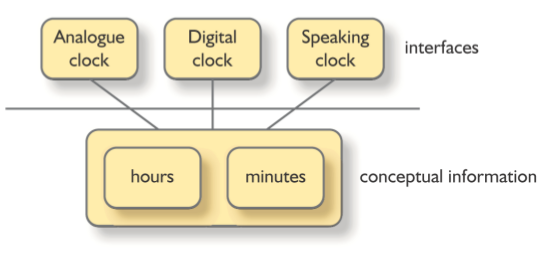
\includegraphics[width=.4\textwidth]{img/ch07_con.png}
	\caption{The same conceptual information can be presented via different physical interfaces.}
	\label{con}
\end{figure}
How is a information presented to the user in term of Form, Structure, and Content/Description? The decision determines which information/action is easier to access and which is more difficult to access. There are various was to arrange windows: Tiled windows afford drag-and-drop methods. Overlapping windows use screen real estate efficiently, but they can become overwhelming. Cascading windows use screen real estate efficiently and can be used to create visual organization. Maximized windows are visually less complex, but they require easy navigation methods to get from window to window. Tabs increase the size of the dialogue by stacking layers on top of each other. Stacked tabs move around to accommodate the different levels and they destroy location consistency.
\subsection{Text and Reading}
The Reading Process can be monitored in term of saccades (quick, jerky eye movements, about 8-10 letters) and fixations (intermittent pauses on areas of interest). Visual and cognitive processing occurs during fixation but not during saccades. If text is difficult to comprehend, if it includes long or unfamiliar words, fixations increase in duration. Reading is a 2-step process:\\
1) distinguish letter or word shapes (only experienced readers recognize word shapes)\\
2) Associate meaning\\\\
Some known human issues concerning text/reading:
\begin{itemize}
\item Readers do not have much trouble reading texts where the letters of the individual words are jumbled, as long as the first and last letter of each word remain in place.
\item Single letters are simpler identifiable if they are in uppercase
\item We read extended text passages more quickly in lowercase than uppercase
\item Lowercase presentation is more common. Lowercase words have more distinctive shapes.
\item Reading a novel is a continuous process. For many other texts we use scanning
\item Reading from screens or paper is different: We often rely on our spatial memory when we search for information (Web-Problem!). On paper, the ability to annotate aids comprehension.
\end{itemize}
In interaction design, text is either used in two ways:
\begin{itemize}
\item Commentary -- Text that informs: The most common form is help text.
\begin{itemize}
\item Contextual help provides immediate assistance to users without requiring them to leave the context in which they are working, such as pop-up menus.
\item Procedural help provides the steps necessary for carrying out a task.
\item Reference help serves as an online reference book.
\item Conceptual help provides background information, feature overviews, or processes
\end{itemize} 
\item Instrumental -- Text that does work: Controls (Buttons, Checkboxes, Radio Buttons, Icons, Hyperlinks) have labels which form one entity with their respective function. E.g. Hypertext links must give unambiguous indications of the target destination.
\end{itemize}
Other Design Issues are Legibility (Age, context determine size, contrast etc.), Readability (comprehension is affected by Line length, Line spacing, Formatting, Margin width, Scrolling and also by grammatical issues, such as semantics and syntax) and \textbf{Physical Factors}:
\begin{itemize}
\item Font size: 9-12pts are equally readable (Dix et al.); several factors affect font size according to Horton:
\begin{itemize}
\item Reading Distance: Greater distances require larger text.
\item Screen Resolution: Smaller text requires greater resolution to keep the characters clear and legible.
\item Text/Background Contrast: Negative contrast is optimal (black type on a white background).
\item Visual Acuity of User: Age, Abilities etc.
\item Type of Reading: Text can be scanned, read word by word, or read character by character
\end{itemize}
\item Line length: affects reading performance but not comprehension. Lines of greater length are read more quickly. People prefer medium line lengths.
\item Margin width: Shorter lines with large margins increase reading performance (Maximal use of white space)
\item Vertical line spacing: The spacing between lines of text (single spacing, double spacing, etc.) is called leading. Double spacing has been shown to improve reading speed. However, it might necessitate a smaller font size to increase the amount of visible information per screen.
\item Alignment: For optimal reading of lengthy texts, right and center alignments should be avoided. Text should also be considered a graphical component of a page.
\item Contrast: Contrast sensitivity decreases significantly with age. Because black and white have the highest contrast the addition of any color will reduce the contrast. Luminance contrast is more significant than color contrast.
\item Scrolling versus paging: Which is better depends on application.
\end{itemize}
\textbf{Fonts}: Serif fonts guide the reader. Thus they are suitable for long text lines e.g. in books. Non-serif fonts are less complex to recognize (less elements), thus they are more suitable for cases where fast recognition is important, e.g. presentation slides. Cursive text is similar to hand written text and requires high-resolution screens. One further distinguished between variable-width and fixed-width fonts. In the latter, each character takes up the same horizontal width ($\rightarrow$ more whitespace in between letters).
There are good (most of them expensive) and cheap fonts (E.g. Arial is a cheap version of Helvetica). Font creation and readability of fonts is a science of its own.

\subsection{Information}
The Information Architecture structures the presented information, thus influencing the conceptualization of the user. Ontologies define the concept of information. How we group things together/ classify them is the concern of taxonomy. Information should be presented consistently (i.e. using one taxonomy), but we know that in practice several taxonomies can coexist.\\
Two general ways for structuring:
\begin{itemize}
\item Coarse-grained: The general information structure provides many objects to be selected. This reduces the number of steps until you reach the object in question. Example: One HTML document containing several sections
\item Fine-grained: There are fine-grained objects, that are reached through a sophisticated, often multi-step process (e.g. through several menus). Example: One HTML document per section
\end{itemize}
How to build information structure: 
\begin{itemize}
\item Volatility: Select an ontology that stays stable, e.g. so you do not have to change your menu logic
\item Size: Decide if moving in an object is more suitable than moving between objects, e.g. scrolling vs. forward-next clicking (experts prefer scrolling)
\item Conceptual / physical mapping: Information must be suitable to all input/output devices ($\rightarrow$ 20 Menu buttons on mobile phone?)
\item Topology: Most important also for Web, determines how easy it is to move through information space (e.g. a Web-Site). Distance is the number of clicks needed for navigation. Direction plays a role for navigation, e.g. an Audio Interface has often only forward navigation
\end{itemize}
In information design it is also important to use one consistent classification scheme, e.g. Alphabetical, Chronological, Geographical (e.g. travel agent: ``Germany''), Topic (e.g. Cars, Repairs), Task-based (``buy a car'',''repair a car''), Audience (Car Buyers), Semantic (Functions, Objects etc. separated)

\subsection{Interaction}
There are many interaction styles: 
\begin{itemize}
\item Command Line: You need to recall information, not recognize it. But it is also simpler to remember words than graphical interface elements. We need a very good concept of use. Steep learning curve, thus better for expert users. Repetition of tasks is simpler. Complexity can be handled easy through concatenation etc. In general faster for complex tasks. But higher error rate, higher cognitive load.
\item Menu-Based Interface: Function can be recognized, position/structure recalled. Menus may be graphical or textual. Much better for seldom used functions, self explanatory. Range of possible options shown $\rightarrow$ constraints. Allows a user to build a concept of the system. Menu Types include Single, Sequential, Hierarchical and Network / Meshed menus.
\item Form Fill-In: Special for gathering strings of information. Linear, not related to navigation. It is important that the users know how long the form will be, and where he is. Errors are problematic, annoy the user. Unambiguous labeling is important to preserve data integrity. Input formats may vary (e.g. how to enter a date?)
\item Wizards/Question and Answer: Form with flow for beginners. Often represents ``most used'' design flow. Present only very restricted information at one time. Very restricted in control flow, thus inappropriate for any input where a great variety of control flows exist. BUT: Today omnipresent in many applications, because most users are beginners at some point (e.g. installation time) for programs. Or always, because of infrequent use.
\item Direct Manipulation/Metaphors (Ben Sheiderman, 1982): Continuous representations of objects and actions of interest with meaningful visual metaphors. Simple physical actions to perform manipulations. Rapid, incremental, reversible actions whose effects on objects are visible immediately. Metaphors are most critical: They allow a user to understand a concept without or with reduced learning, often using real-world associations. However, they are not always consistent and simplifying. Also, different people have various concepts for the same objects. Touch interaction is also a form of direct manipulation.
\item Web Navigation
\item Three-Dimensional Environments
\item Zoomable Interface
\item Natural Language
\end{itemize}
\textbf{Object-Action model}: The user first selects an object and then selects the action to be performed on the selected object (e.g. MAC user interface).\\\\
\textbf{Action-Object model}: The user first selects an action to be performed and then selects the objects on which this action will be performed (e.g. typical Windows usage).



\end{document}


%%% Local Variables:
%%% mode: latex
%%% TeX-master: t
%%% End: